%!TEX TS-program = xelatex
%!TEX encoding = UTF-8 Unicode

%============ Logs ===========================
\newcommand{\version}{ver 2.1}
%=============================================

\documentclass{mahidol_thesis}
%====== Add the packages here ===============
\usepackage{multirow}
\usepackage[table,xcdraw]{xcolor}
\usepackage{subcaption}
\usepackage{lscape}
\usepackage{amsmath}
\usepackage{lipsum} %Generate dummy text for testing
%====== List of Coding Color Style ==============
\definecolor{codegreen}{rgb}{0,0.6,0}
\definecolor{codegray}{rgb}{0.5,0.5,0.5}
\definecolor{codepurple}{rgb}{0.58,0,0.82}
%\definecolor{backcolour}{rgb}{0.95,0.95,0.92}
\definecolor{backcolour}{rgb}{1,1,1}
%=======================

%====== Path to Figure Directories ===============
\graphicspath{{./figures/chap1/}{./figures/chap2/}{./figures/chap3/}{./figures/chap4/}{./figures/chap5/}{./figures/chap6/}{./figures/appendix/}}


%%%%%%%%%%%%%%%%%%%%%%%%%%%%%%%%%%%%%%
%Thesis Meta Data (edit each field)
%%%%%%%%%%%%%%%%%%%%%%%%%%%%%%%%%%%%%%
%Thesis Title 
\newcommand{\thesisTitle}{Motorbike Image Recognition using YOLO}
\newcommand{\thesisTitleTH}{ชื่อวิทยานิพนธ์}

%Thesis Keywords
\newcommand{\thesisKeywordsTH}{ ลาเท็ก / วิทยานิพนธ์ (\~{}5 คำ)}
\newcommand{\thesisKeywords}{ LaTeX / Thesis (\~{}5 words)}

\newcommand{\totalPageTH}{30}   %Total pages (See. the total number in English Acknowledgement Page then fill up here!)
%\newcommand{\totalPageTH}{\pageref{LastPage}}

%First Author name
\newcommand{\thesisFirstTitleName}{Mr.}
\newcommand{\thesisFirstAuthorName}{Phasin}
\newcommand{\thesisFirstAuthorLastName}{Ploypicha}
\newcommand{\thesisFirstTitleNameTH}{นาย}
\newcommand{\thesisFirstAuthorNameTH}{ชื่อผู้แต่ง}
\newcommand{\thesisFirstAuthorLastNameTH}{นามสกุลผู้แต่ง}
\newcommand{\thesisFirstAuthorID}{123567}
\newcommand{\thesisFirstAuthorBD}{28 March 2003}
\newcommand{\thesisFirstAuthorBP}{Bangkok, Thailand}
\newcommand{\thesisFirstAuthorHC}{Mahidol International College}
\newcommand{\thesisFirstAuthorTel}{111 111 1111}
\newcommand{\thesisFirstAuthorEmail}{phasin.plo@student.mahidol.edu}

%Second Author name
\newcommand{\thesisSecondTitleName}{Mr. }  %Comment all if you don't have second author
\newcommand{\thesisSecondAuthorName}{Piyakorn}
\newcommand{\thesisSecondAuthorLastName}{Rodthanong}
\newcommand{\thesisSecondTitleNameTH}{นางสาว }
\newcommand{\thesisSecondAuthorNameTH}{ชื่อผู้แต่ง}
\newcommand{\thesisSecondAuthorLastNameTH}{นามสกุลผู้แต่ง}
\newcommand{\thesisSecondAuthorID}{2345678}
\newcommand{\thesisSecondAuthorBD}{15 May 2003}
\newcommand{\thesisSecondAuthorBP}{Bangkok, Thailand}
\newcommand{\thesisSecondAuthorHC}{Mahidol International College}
\newcommand{\thesisSecondAuthorTel}{222 222 2222}
\newcommand{\thesisSecondAuthorEmail}{piyakor.rod@stdent.mahidol.edu}

%Third Author name
\newcommand{\thesisThirdTitleName}{Mr.}   %Comment all if you don't have third author
\newcommand{\thesisThirdAuthorName}{Sopon}
\newcommand{\thesisThirdAuthorLastName}{Pleangnoi}
\newcommand{\thesisThirdTitleNameTH}{นาย}
\newcommand{\thesisThirdAuthorNameTH}{ชื่อผู้แต่ง}
\newcommand{\thesisThirdAuthorLastNameTH}{นามสกุลผู้แต่ง}
\newcommand{\thesisThirdAuthorID}{33333333}
\newcommand{\thesisThirdAuthorBD}{03 March 2002}
\newcommand{\thesisThirdAuthorBP}{Bangkok, Thailand}
\newcommand{\thesisThirdAuthorHC}{Mahidol International College}
\newcommand{\thesisThirdAuthorTel}{333 333 333}
\newcommand{\thesisThirdAuthorEmail}{Sopon.pln@student.mahidol.edu}

%Fourth Author name
%\newcommand{\thesisFourthTitleName}{Mr.}   %Comment all if you don't have fourth author
%\newcommand{\thesisFourthAuthorName}{Firstname4} \n
%\newcommand{\thesisFourthAuthorLastName}{Lastname4}
%\newcommand{\thesisFourthTitleNameTH}{นาย}
%\newcommand{\thesisFourthAuthorNameTH}{ชื่อผู้แต่ง4}
%\newcommand{\thesisFourthAuthorLastNameTH}{นามสกุลผู้แต่ง4}
%\newcommand{\thesisFourthAuthorID}{4444444}
%\newcommand{\thesisFourthdAuthorBD}{04 April 2002}
%\newcommand{\thesisFourthAuthorBP}{Bangkok, Thailand}
%\newcommand{\thesisFourthAuthorHC}{Mahidol International College}
%\newcommand{\thesisFourthAuthorTel}{444 444 4444}
%\newcommand{\thesisFourthAuthorEmail}{FourthEmail@gmail.com}

%Month, year and date of thesis publication
\newcommand{\thesisGradDateTH}{15 กรกฎาคม 2567}  %Graduate Date/Month/Year
\newcommand{\thesisGradDate}{July 25, 2025} %Graduated Year
\newcommand{\thesisAcademicYear}{2025} %Academic Year
\newcommand{\thesisAcademicYearTH}{๒๕๖๖} %Academic Year

%Department
\newcommand{\thesisDepENG}{Computer Engineering}
\newcommand{\thesisDepTH}{วิศวกรรมคอมพิวเตอร์}

%Advisor name
\newcommand{\thesisAdv}{Dr. Mingmanas Sivaraksa }  %with title name
\newcommand{\thesisAdvTH}{ดร. ชื่อที่ปรึกษา นามสกุลที่ปรึกษา}  %with title name
\newcommand{\advDegree}{Ph.D. (Information Engineering),\\ Ph.D. (Computer Innovation Engineering)}

%Thesis Committees
\newcommand{\Chair}{\thesisAdv}
\newcommand{\ChairDegree}{\advDegree}
\newcommand{\committeeI}{Committee 1}
\newcommand{\committeeIDegree}{Ph.D. (Computer Engineering)}
\newcommand{\committeeII}{Committee 2}
\newcommand{\committeeIIDegree}{Ph.D. (Computer Engineering)}
\newcommand{\committeeIII}{Committee 3}
\newcommand{\committeeIIIDegree}{Ph.D. (Computer Science)}

\begin{document}
	%---- Cover Page Section ------
	\coverpageENG
	\coverpageENGTwo
	\entitlepageOne
	\entitlepageTwo
	%---- Front Page Section ------
	\pagestyle{front}
	\frontmatter
	\biography
	\acknowledgement{acknowledgement.tex}
	\abstractTH{abstractTH.tex}
	\abstractENG{abstractENG.tex}
	\tableofcontents
	\newpage
	\listoftables
	\newpage
	\listoffigures
	%---- Body -----
	\pagestyle{chapter}
	\mainmatter
	\pagestyle{fancy}
	\chapter{INTRODUCTION}

\section{Background}
Urban traffic congestion and road safety, particularly for motorbikes, remain major issues. Motorcycles, due to their mobility, contribute greatly to traffic flow. However, they are also prone to violations, such as not wearing helmets or using the wrong lane, which increase the chance of an accident. Traditional traffic management systems lack the ability to detect and address such specific breaches in real time.

AI technologies, like as YOLO, a deep learning model for object detection, have showed potential in traffic surveillance but have not yet been routinely used to identify helmet use or lane breaches. Previous research has shown that YOLO is good for vehicle detection, but there is a gap in its use for targeted motorbike detection and safety compliance.

This research seeks to close this gap by utilising YOLO to detect motorcycles, check for helmet use, and identify lane violations. By focussing on these critical aspects, the system will improve road safety and aid in more effective traffic enforcement.

\section{Objective}
\begin{enumerate}
	\item To detect motorbike, person, helmet and non-helmet user.
	\item Count motorbike, person, helmet and non-helmet users efficiently.
	\item Upload system up to university's server.
\end{enumerate}

\section{Scope}
\begin{enumerate}
    \item Develop system to detect motorbike, person, hemet and non-helmet user.
    \item Display annotated video.
    \item  Count all the essentails and display real time.
    \item University server running on system efficiently.
 

\end{enumerate}

\section{Expected Results}
\begin{enumerate}
	\item To reduce illegal activities of riders.
	\item To ensure both safety of rider and pedestrian.
	\item To spraed safety awareness.
	\item Has more than 80 percent accuracy .
\end{enumerate}

\section{Timeline}
\newcolumntype{L}[1]{>{\raggedright\let\newline\\\arraybackslash\hspace{0pt}}m{#1}}
\newcolumntype{C}[1]{>{\centering\let\newline\\\arraybackslash\hspace{0pt}}m{#1}}
\newcolumntype{R}[1]{>{\raggedleft\let\newline\\\arraybackslash\hspace{0pt}}m{#1}}	

\begin{table}[!ht]
	\footnotesize
	\sloppy
	\centering
	\caption{Project Timeline}
	\label{tab: your-table} %for cross-reference
	\begin{tabular}{|p{2.15cm}|c|c|c|c|c|c|c|c|c|c|c|c|}
		\hline
	\multicolumn{1}{|c|}{}& \multicolumn{12}{c|}{\textbf{Timeline}} \\ \cline{2-13} 
	\multicolumn{1}{|c|}{}& \multicolumn{9}{c|}{\textbf{2024}} & \multicolumn{3}{c|}{\textbf{2025}} \\ \cline{2-13} 
	\multicolumn{1}{|c|}{\multirow{-3}{2cm}{\textbf{Plan}}} & \textbf{Oct} & \textbf{Nov} & \textbf{Dec} & \textbf{Jan} & \textbf{Feb} & \textbf{Mar} & \textbf{Apr} & \textbf{May} & \textbf{Jun} & \textbf{July} & \textbf{Aug} & \textbf{Sep} \\ \hline
	Wrting Proposal &
	\cellcolor[HTML]{000000} &
	\cellcolor[HTML]{000000} & 
	\cellcolor[HTML]{000000} & & & & & & & & & \\ \hline
	Review Paper and Methodology& & &
	\cellcolor[HTML]{000000} & 
	\cellcolor[HTML]{000000} & & & & & & & &\\ \hline
	Data Gathering & &  & &
	\cellcolor[HTML]{000000} &
	\cellcolor[HTML]{000000} & & & & & & & \\ \hline
	Start Training Model & & & & &
	\cellcolor[HTML]{000000} &
	\cellcolor[HTML]{000000} &  
	\cellcolor[HTML]{000000} & & & & & \\ \hline
	Finalize  Training Model & & & & & & & &
	\cellcolor[HTML]{000000} &
	\cellcolor[HTML]{000000} & & & \\ \hline
	Prepare University Server Specs& & &  & & & & & &  
	\cellcolor[HTML]{000000} & 
	\cellcolor[HTML]{000000} & &\\ \hline
	Deploy and connect to database & & & & & & & & & & &  
	\cellcolor[HTML]{000000} & \\ \hline
	Presentation & & & & & & & & & & & & \cellcolor[HTML]{000000} \\ \hline
	
	\end{tabular}
\end{table}
	\chapter{LITERATURE REVIEW}

The papers in the literature review are used as a foundation to guide, the thesis, this included inspiration, the methodoly, and expected results.

\section{Video Image Recognition of Car Track Characteristics at Intersections \cite{paper_1}} 

The system relies on machine learning algorithms to interpret video data in real-time, helping to optimize traffic signal control, reduce congestion, and enhance safety. The study emphasizes its application in intelligent transportation systems and urban traffic flow optimization.

The use of YOLOv8, a popular deep learning model for object detection, because it offers a balance of speed and accuracy. YOLOv8 is efficient in processing real-time video streams, which is crucial for tracking vehicles at intersections. It excels in recognizing objects (like cars) in complex environments, and its architecture allows it to detect vehicles quickly while maintaining high precision.

\newpage
\section{A Lightweight Remote Sensing Small Target Image Detection Algorithm Based on Improved YOLOv8 \cite{paper_2}}
The authors optimize the YOLOv8 architecture by refining the feature  process and introducing techniques like multi-scale detection, anchor box adjustments, and a better feature fusion method. This helps the algorithm perform better with small targets.
ensuring more accurate detection without significantly increasing computational cost.

they conclude that, this makes it suitable for real-time applications in remote sensing, where detecting small objects like vehicles, ships, or buildings in satellite imagery is critical. The enhancements lead to better precision and recall.


\section{Traffic Detection and Enhancing Traffic Safety: YOLO V8 Framework and OCR for Violation Detection Using Deep Learning Techniques \cite{paper_3}}
The YOLOv8 algorithm is a deep learning model that uses a convolutional neural network (CNN) to detect and classify objects in input images. It uses bounding box regression and class prediction to identify objects and assign class probabilities. 

The model is pre-processed by converting the input video into frames, extracting features, and detecting objects. The YOLOv8 model then uses a grid to track objects, predicting bounding boxes and class probabilities. The model is fine-tuned on specific object classes and implemented for tracking, counting, and speed estimation.

This project consists of two main modules: one for vehicle count and speed detection, which uses a dataset of 800 images and video clips, and the other for number plate recognition. The first module uses computer vision techniques to accurately count vehicles and calculate speeds. The second module uses a Roboflow website dataset to extract license plate information, useful for applications like parking management and traffic monitoring. 

This project aims to create two modules with distinct functions in traffic monitoring. The number plate recognition module enhances functionality for recognizing and tracking vehicles based on their number plates, while the vehicle count and speed detection module provides insights into traffic flow and speed trends.

The study on traffic detection using the YOLOv8 framework and Optical Character Recognition (OCR) has shown promising results. The system accurately detects traffic violations in real-time, while OCR enhances its ability to identify and classify violations like illegal parking or speeding.

YOLOv8 and OCR provides a robust solution for automating violation detection processes, demonstrating the effectiveness of deep learning methodologies in enhancing traffic safety and enforcing traffic regulations.


\section{Smart Traffic Management System for Efficient Mobility and Emergency Response \cite{paper_4}}
The proposed solution combines AI with real-time data analytics to improve traffic light management. It incorporates real-time congestion response, algorithmic optimization, data-driven decision making, and feedback loop integration. 

The system uses a vast dataset of lane-specific traffic information to inform real-time adjustments. The Traffic Light Control System (OF) is activated, and the dataset undergoes preprocessing to ensure compatibility with the algorithms. A predictive model is trained using machine learning techniques, and a feedback loop is implemented to continuously evaluate the effectiveness of the decisions. 

The AI system also optimizes traffic flow during emergencies, adjusting timings to prioritize passage and ensure smooth traffic flow. This innovative approach aims to alleviate congestion and improve overall traffic flow, ultimately leading to sustainable and safer cities.

\newpage
\section{Utilizing Image Processing and the YOLOv3 Network for Real-Time Traffic Light Control \cite{paper_5}}
The paper presents the creation of a traffic light control system which is aimed at relieving congestion in urban areas. The system is designed based on the YOLOv3 object detection algorithm and is capable of counting both vehicles and pedestrians at intersections in real time using a Jetson Nano board for data processing. The research further shows that traffic lights can be controlled by taking into consideration factors such as the number of vehicles that have stopped, the number of vehicles that are crossing over and the number of pedestrians thereby enhancing the efficiency of the system which in turn reduces negative impacts on the environment.

The authors note the cost entailed in relief from congestion in UK being in the region of £37.7 billion per year and admonish that such inefficient delay is caused by the inadequate control of traffic lights that energy loss is also the outcome of that inefficient management of the traffic signal is responsible. The developed system loks set to achieve average precision with average vehicle counting for 95 percent as supported by this research.



\newpage
\section{Research on Vehicle Lane Change Warning Method Based on Deep Learning Image Processing \cite{paper_6}}
The paper presents the progress in work which is falling into the category of the development of the low-cost lane-changing warning system which works in the efforts to improve driving safety through monocular camera and deep learning algorithms. The main aim of the study is to detect when there is a pole vehicle-user behavior who would be changing the existing lane as this is paramount to mitigate risk of collision, consequently enhance safety of roads.

As a result, the authors enhanced the Mask Region-based Convolutional Neural Network (Mask R-CNN) aiming towards a vehicle target seeker. They used the K-means clustering technique to identify appropriate proportions of anchor frames for vehicle targets, which facilitated more precise candidate box generation without degrading the performance of the network. This led to introduction of a fresh anchor set and mAP increased by about 2.6 percent thanks to about 26 percent in the mean average precision improvement.

The system was trained in a vernacular fashion with a full with 66,389 vehicle targets which were adequately annotated for target annotation assuring their appropriate performance. The authors performed various evaluations and recorded an accuracy of 94.5 percent for detection of lane changing after identifying and validating marked images of lane changing sequences. This high accuracy demonstrates the effectiveness of the proposed system in real time applications.


\newpage
\section{Summary}
The reviewed studies highlight innovative uses of AI and deep learning for traffic management and safety. One study employs the YOLOv8 framework and Optical Character Recognition (OCR) to detect traffic violations in real-time, using modules for vehicle counting, speed estimation, and license plate recognition, achieving effective enforcement of traffic regulations. Another study integrates AI with real-time analytics to optimize traffic light control, dynamically responding to congestion and prioritizing emergency vehicles, thereby improving urban mobility and sustainability. Similarly, a traffic light control system based on YOLOv3 counts vehicles and pedestrians at intersections, achieving 95 percent accuracy in optimizing traffic flow and reducing urban congestion. Lastly, a lane-change warning system utilizing Mask R-CNN and K-means clustering achieves 94.5 percent accuracy in detecting lane changes, offering a cost-effective solution for collision risk mitigation and enhanced road safety. These approaches collectively demonstrate the transformative potential of AI in traffic management.








	\chapter{METHODOLOGY}
\section{System Design}

	The purpose of the helmet detection system is to track helmet use from CCTV footage on a college campus. Data preparation, model training, and counting implementation are the three primary phases of the system. The first step involves converting campus CCTV video footage into image frames, which are subsequently labelled with helmet and unhelmeted head information using Roboflow. A customised YOLOv8 object detection model that is tuned for real-time performance is trained using the annotated dataset. After training, the model is incorporated into a real-time system that recognises and categorises heads and helmets by processing incoming video frames. In order to provide real-time statistics that facilitate safety compliance monitoring, a counting mechanism is integrated to monitor the quantity of helmets and heads seen within a designated area of interest.
	

\begin{figure}[H] % Optional: [H] requires \usepackage{float}
	
	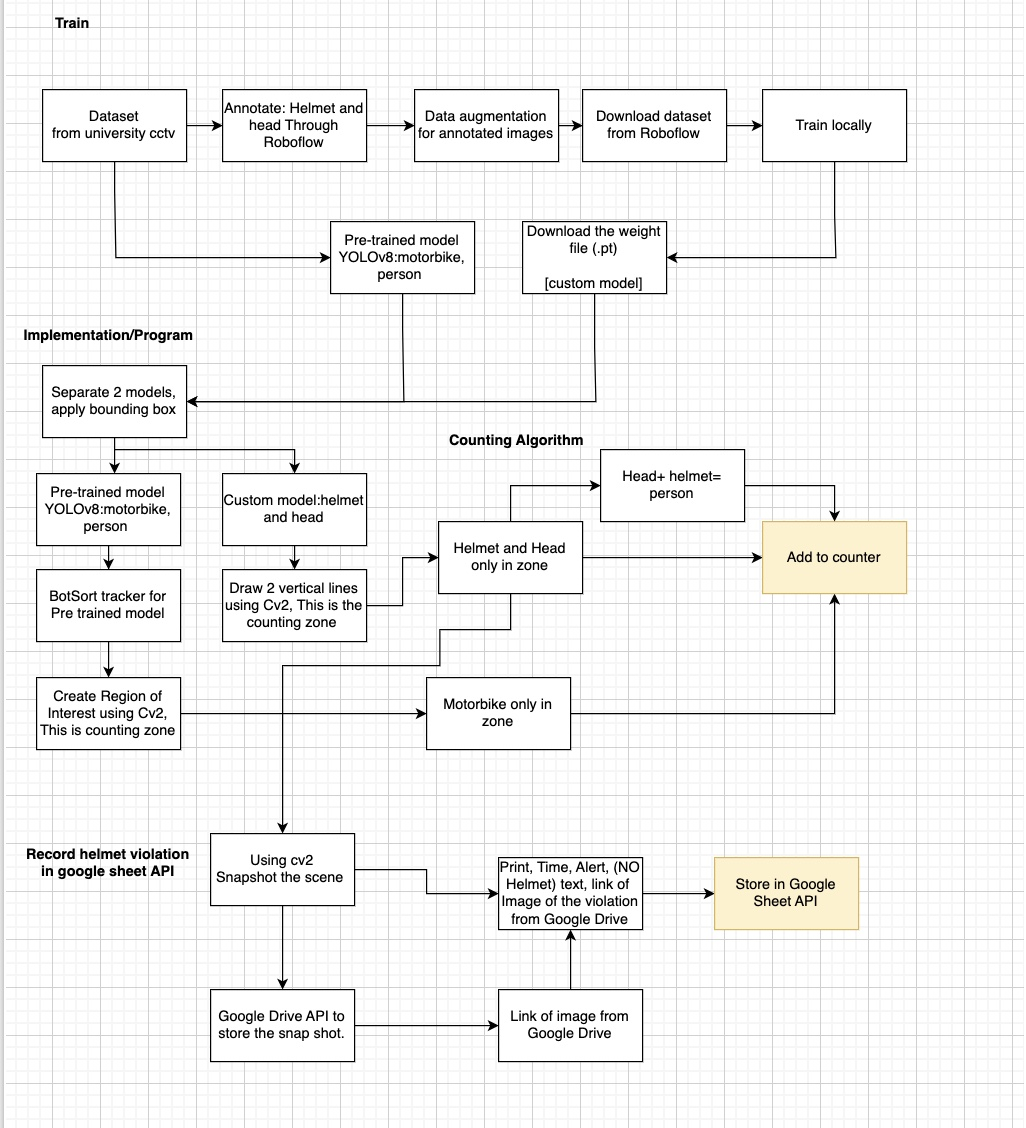
\includegraphics[width=1\textwidth]{flowchart.jpg}
	\vspace{0.5em}
	\noindent\textbf{Figure 3.1} \\
	\caption*{} % Optional: if you want a caption, otherwise keep empty
	
	
\end{figure}

	 The flowchart illustrates the overall workflow of the system. It begins first obtaining the dataset, we obtain them through the cctv footage of the university camera. Specifically spliting the video footages into 3 frames per second using Roboflow. Then annotate each frames splited, the annoated items are helmet and head, then using data augmentations from Roboflow. Then we can downlaod the datasets. Finally, using dataset downloaded we can train locally through data.yaml, the data augmentations details are to be specified in Chapter 3. After the training we will receive the weighted .pt file, the file is the model that will be used in the system in conjunction with the pre-trained model from YOLOv8. The Implementation phase is to apply the models, work with the video stream input. The bounding box and region of interest made from cv2. Using these zone we speparate the counting zone for helmet, head, and another zone to count person and helmet. As for the person we decided to count the head and the helmet to total to person as there are issues about the camera angel limiting the accuracy of the person detection. 
	
	After implementing the program with the model, we use cv2 to take snapshot of the frame as when helmet violation occur. The system links and uses Google API, to store the detection evidence of the scenario. The Google Sheet API will append new rows each time a head detection occur.  The image are visible, and stored by Google Drive API, to check the instances where it happens.
	
\section{Data}
Dataset: videos of riders wearing and not wearing helmets, collected from local sources which is gate six Mahidol University CCTV camera. Videos will then be split in Roboflow which allow custom annotation and training.
\newline
\newline
Annotations: Create two classes. first class containing the bouding box of helmet user only and the second class containing head(which is non-helmet user.)
\newline
Preprocessing: Includes resizing images to 640x640 pixels, normalizing pixel values, and applying augmentations (e.g., rotation, scaling, and brightness adjustments).

\newpage
\section{Custom Model}
\textbf{YOLOv8 Architecture:}
The YOLOv8 architecture was selected for this project due to its state-of-the-art performance in object detection, offering a balance between real-time inference speed and high accuracy. YOLOv8 (You Only Look Once version 8), developed by Ultralytics, is known for its streamlined architecture and improved detection performance over its predecessors (e.g., YOLOv5, YOLOv7), particularly in low-light or occluded environments—conditions often encountered in real-world surveillance footage. Specifically for this project, YOLOv8 is supported by Roboflow, a tool important for training and annotating helmet and head classes easily. Additionally YOLOv8 was easier to set up and supported by developers and communities in a larger scale than other YOLO versions. This will be essentials in debugging and implementing additional tools like trackers. 

Despite the availability of newer object detection models such as YOLO-NAS or YOLOv9, YOLOv8 remains a highly reliable and widely supported choice. In this project, YOLOv8 was used to create a custom-trained model that focuses on five specific object classes: motorcycles, helmets, crosswalks, pedestrians, and lanes. However, the two most critical objects for our safety analysis—helmet and head—were prioritized in both annotation and evaluation.


\begin{center}
	\begin{minipage}{0.45\textwidth}
		\centering
		
\includegraphics[width=\linewidth]{roboflow.png}
		\vspace{0.5em}
		
		\textbf{Figure 3.3.1: Roboflow Image}
	\end{minipage}
	\hfill
	\begin{minipage}{0.45\textwidth}
		\centering
		
\includegraphics[width=\linewidth]{yolo.png}
		\vspace{0.5em}
		
		\textbf{Figure 3.3.2: YOLO Image}
	\end{minipage}
\end{center}

To obtain the custom model for "head", and "helmet" detection we must first upload the datasets into Roboflow website in figure 3.1. Roboflow will allow users to specifically annotate desired classes, which after annotating said datasets, we can download directly from Roboflow the annotated datasets which we can train locally. Training can be done localy or through Google Collab. However due to limitations we used Vistual Studio as a medium to train the datasets from Roboflow. 

\newpage
	
\noindent\textbf{Training Process:} As for our goals the training processes for our custom YOLOv8 model consisted of several key stages, summarized below:

\begin{itemize}
	 \item \textbf{Data Collection:} The dataset was compiled from real CCTV footage recorded on campus at Mahidol University’s Faculty of Engineering. The footage was collected over a span of seven days during the morning rush hour (8:00–10:00 AM), totaling approximately two hours. This time window was chosen to capture peak motorcycle and pedestrian traffic for accurate helmet usage monitoring.  The image below is an example of a snapshot from the dataset, the actually dataset is a video as mention.
\begin{center}
	\includegraphics[width=0.5\textwidth]{Datasets.png}
	
	\vspace{0.5em}
	\textbf{Figure 3.3.3: Dataset Image}
\end{center}
	 
	\item \textbf{Frame extracgtion:} Using the cv2 module from OpenCV, video footage was processed and extracted into still frames. To ensure computational efficiency while retaining sufficient information, frames were sampled at a rate of 3 frames per second (FPS). The extracted images were then uploaded to Roboflow, a computer vision dataset platform, for annotation and augmentation. However for Roboflow they provide a function to slpit the frames within the website and we will be extracting them with Roboflow instead. In the figure below is an example of frame extraction function after uploading the datasets into Roboflow. Extracting the video datasets into frames, means that we can annotate each frames specifically we have three frames across one second. This is to also ensure that we do not have to much datasets, and it also depends on how much the desire classes appears on the videos. For our case there are enough objects across three frames per second to annotate.
	\begin{center}
		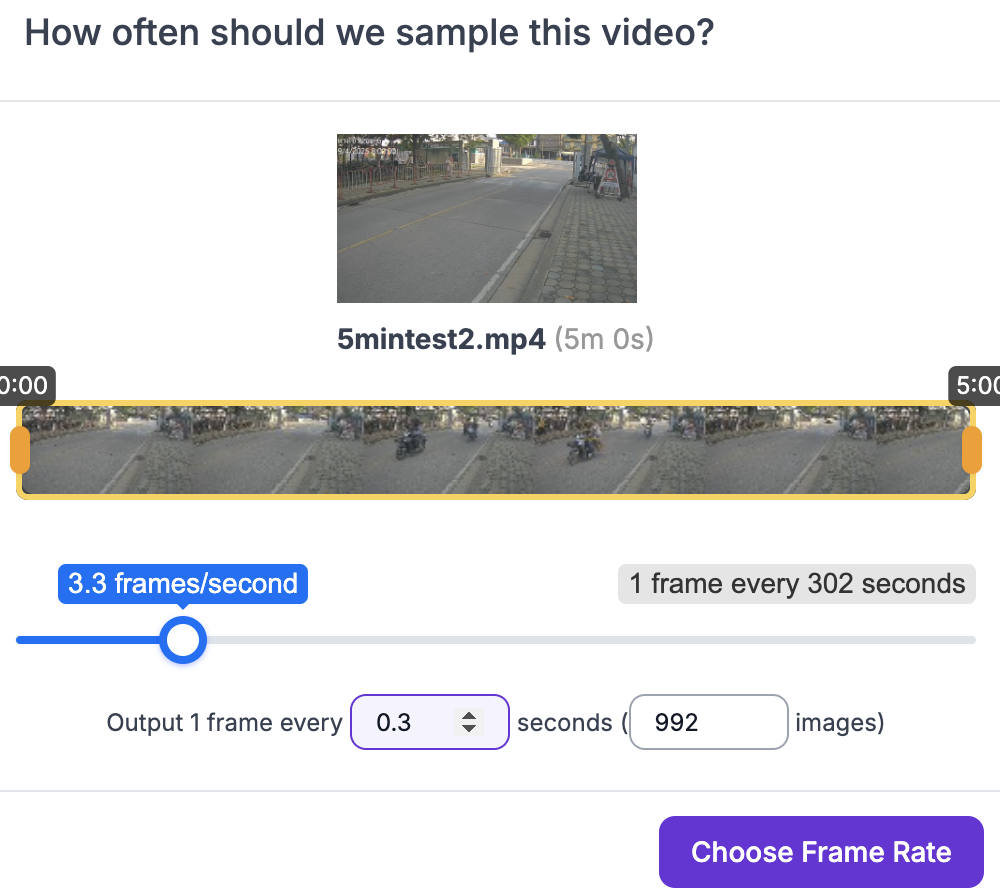
\includegraphics[width=0.5\textwidth]{Frameex.png}
		
		\vspace{0.5em}
		\textbf{Figure 3.3.3: Frame Extraction Image}
	\end{center}
	
	\item\textbf{Annotation:} Within Roboflow, bounding boxes were manually drawn around the target objects—specifically helmets and heads—to create accurate ground truth data for supervised learning. Annotations were carefully reviewed to ensure consistency, especially in challenging cases such as partial occlusions or non-standard helmet designs. The images belows show an example how we draw the bounding boxes for the classes. Drawing the bouding box this way minimizes detection errors and allows the YOLOv8 custom model to focus on the objects more precisely. We encourage to draw the bounding box as close to the objects as possible.
		\begin{center}
		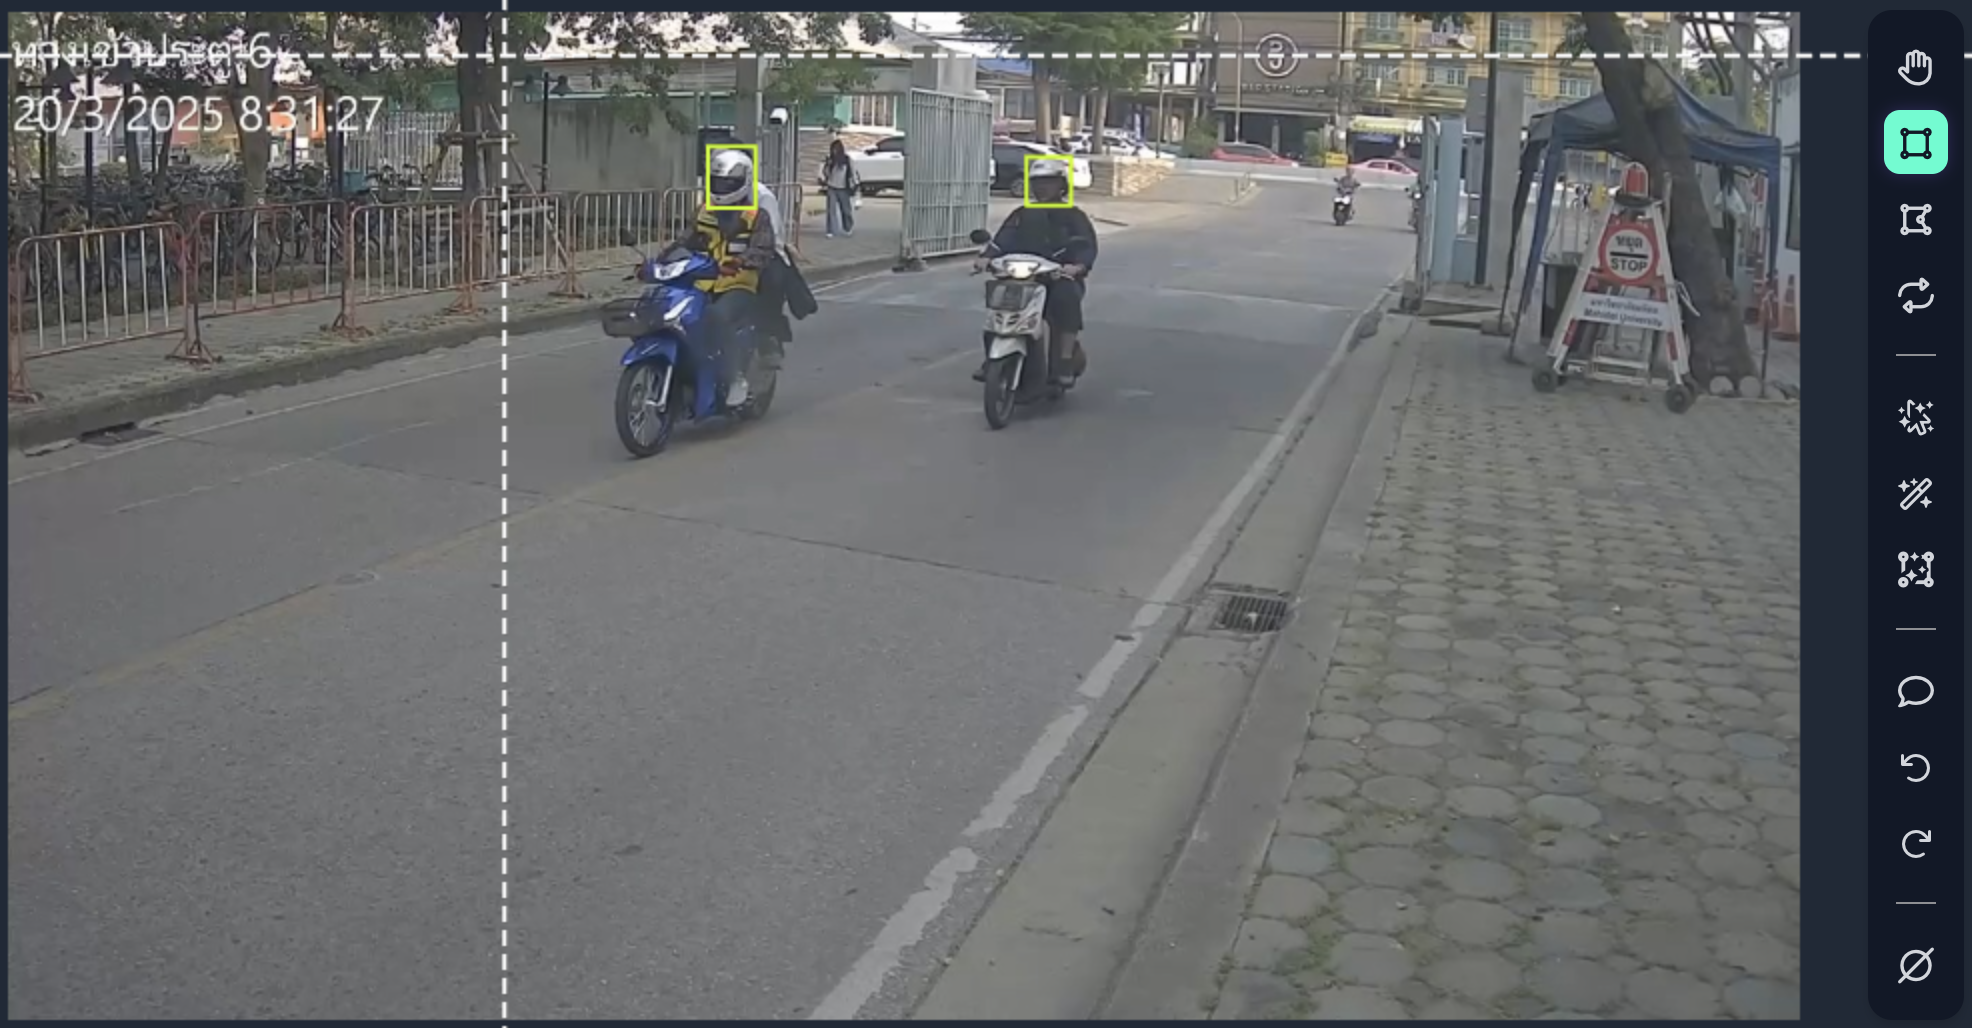
\includegraphics[width=0.8\textwidth]{Anotate.png}
		
		\vspace{0.5em}
		\textbf{Figure 3.3.4: Annotation Image}
	\end{center}
	\newpage
	\item \textbf{Dataset Splitting:}  The annotated dataset was divided into training, validation, and testing sets with a ratio of 70\% training, 20\% validation, and 10]\% testing. This split was chosen to ensure sufficient training samples while preserving a robust validation set to monitor overfitting and a separate test set for unbiased evaluation. Using this data split is widely uses apporach in machine learning as it offers balnce between training, validation, and testing. 70\% of the data use to train allows it to learn patterns from the annotation effectively. It is effieicent and enough for pattern recognition. The 20\% is very important as becuase as this portion is used to check how well the model is learning. Additionally to help tune with the hyperparameters and prevent overfitting. Overfiting occurs when a  model memorizes the training data too well and fails to perform on new, unseen data.  Lastly the 10\% is reserved for testing, for unbaised evaluation of the model. The split ensures thatt the model has enough data to learn, and adjust. This process will occur after completing the annotation process.		
		\begin{center}
		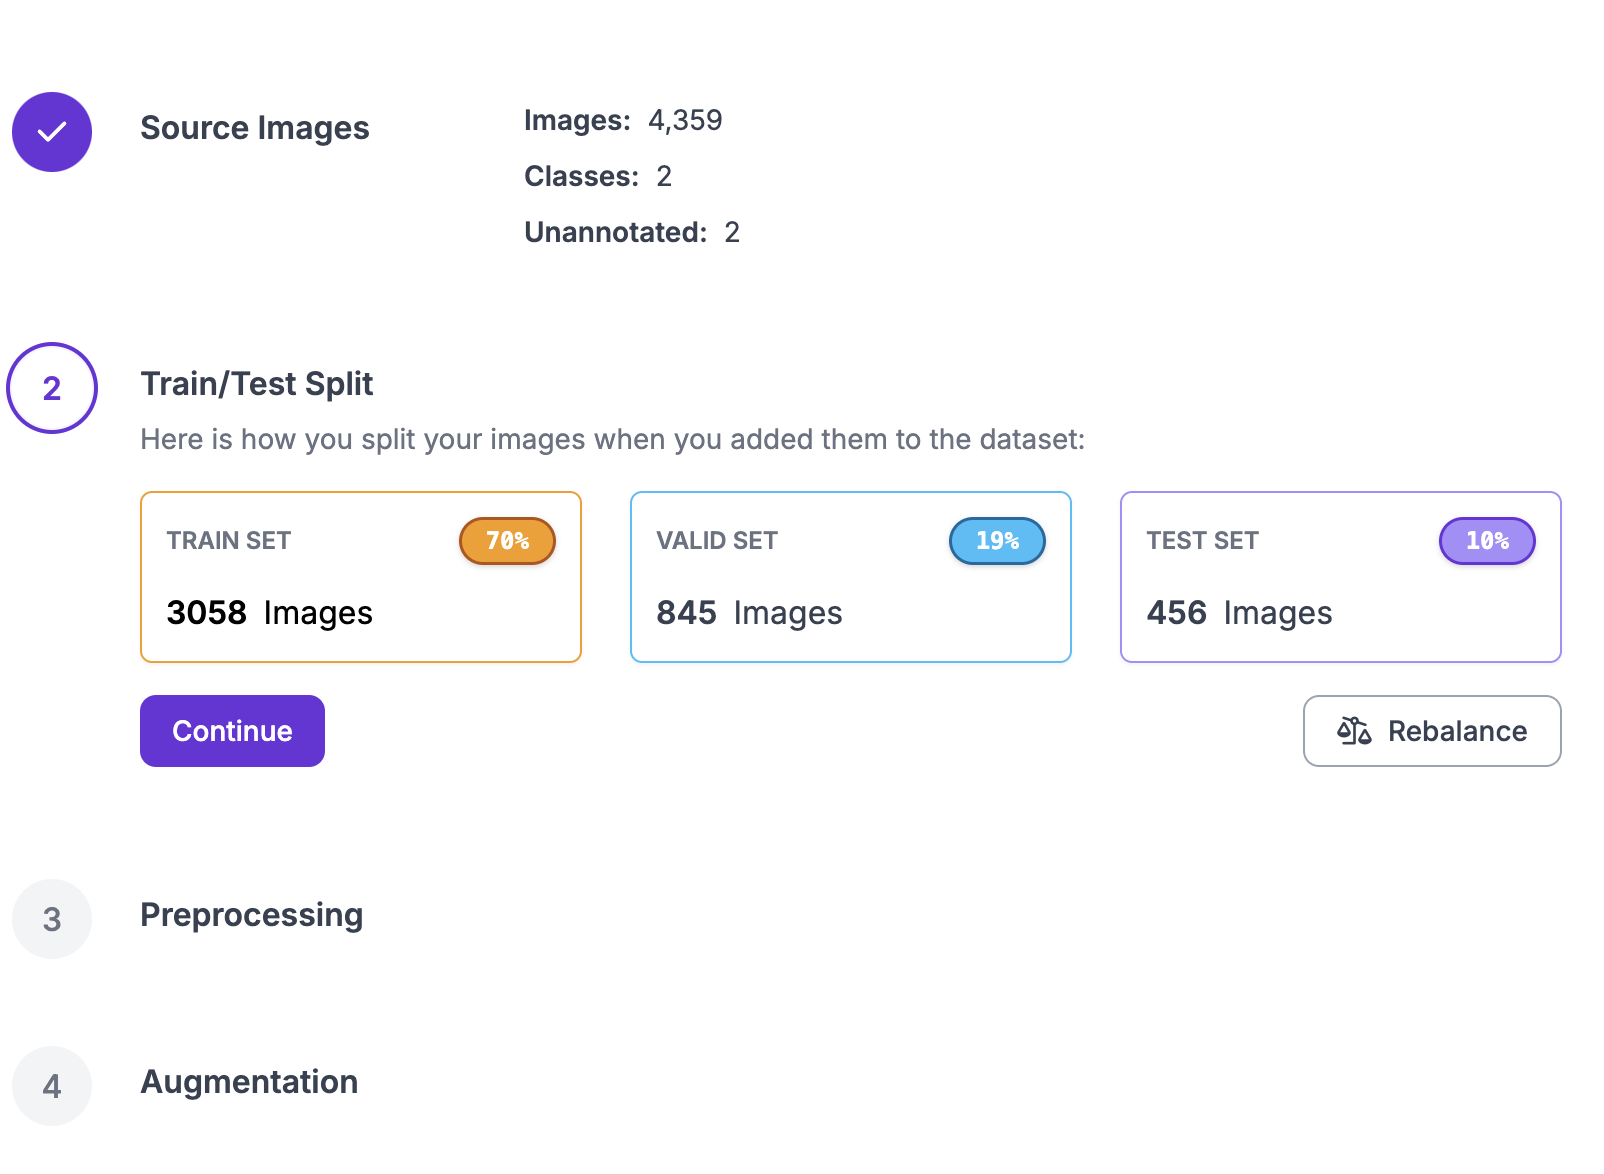
\includegraphics[width=0.8\textwidth]{Split.png}
		
		\vspace{0.5em}
		\textbf{Figure 3.3.5: Spliting Datasets Image}
	\end{center}
	At this step we can also augmentate our data through data augmentation from Roboflow seen in Figure 3.3.5. Data augmentation techniques applied are horizontal flipping, contrast enhancement, and brightness variation were applied to improve the model’s robustness to environmental variations such as lighting conditions or camera angles.
			\begin{center}
		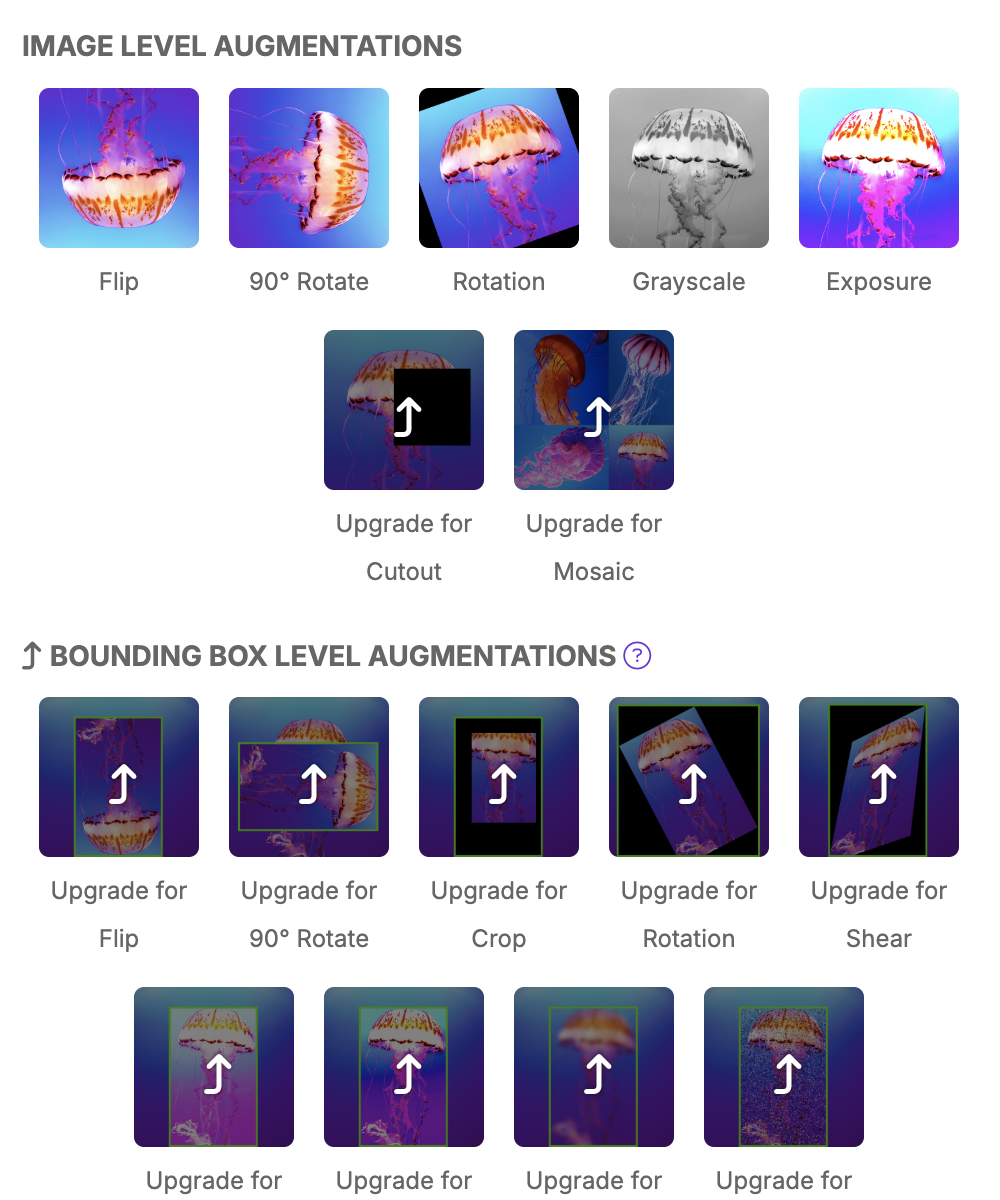
\includegraphics[width=0.8\textwidth]{Augmentation.png}
		
		\vspace{0.5em}
		\textbf{Figure 3.3.6: Augmentation Image}
	\end{center}
	
	\item \textbf{Data Configuration and Training:} Aftering Spliting the data we can download the dataset files from Roboflow. The file will be splited to 70/20/10, train, validate, test. A data.yaml file will have to be  configured to specify class names, dataset paths, and other training parameters. The file is then imported imported into Visual Studio Code (VS Code) for model development and training using the Ultralytics YOLOv8 framework. The images below shows how data.yamlfile is set up.
				\begin{center}
		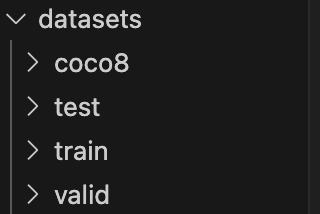
\includegraphics[width=0.8\textwidth]{Files.png}
		
		\vspace{0.5em}
		\textbf{Figure 3.3.7:  Files from downloaded Dataset }
	\end{center}
	 The detailedconfigurations needed used inside data.yaml is located in the Hyperparameter section.
	 Hyperparameters, such as learning rate and non-maximum suppression (NMS) thresholds, were tuned for optimal performance.  After applying the hyparameters, we can start the training through the data.yaml file. After the training has been finish, the wieghted model files will be created in runs/detect. Select the .pt files as a yolo model this will be the model that we will use after all the steps above are complete. For our project be have a total of 4,359 images that are annotated for custom model. The image belows shows the data.yaml content. We will use this to obtain a custom weighted  .pt file.
	 				\begin{center}
	 	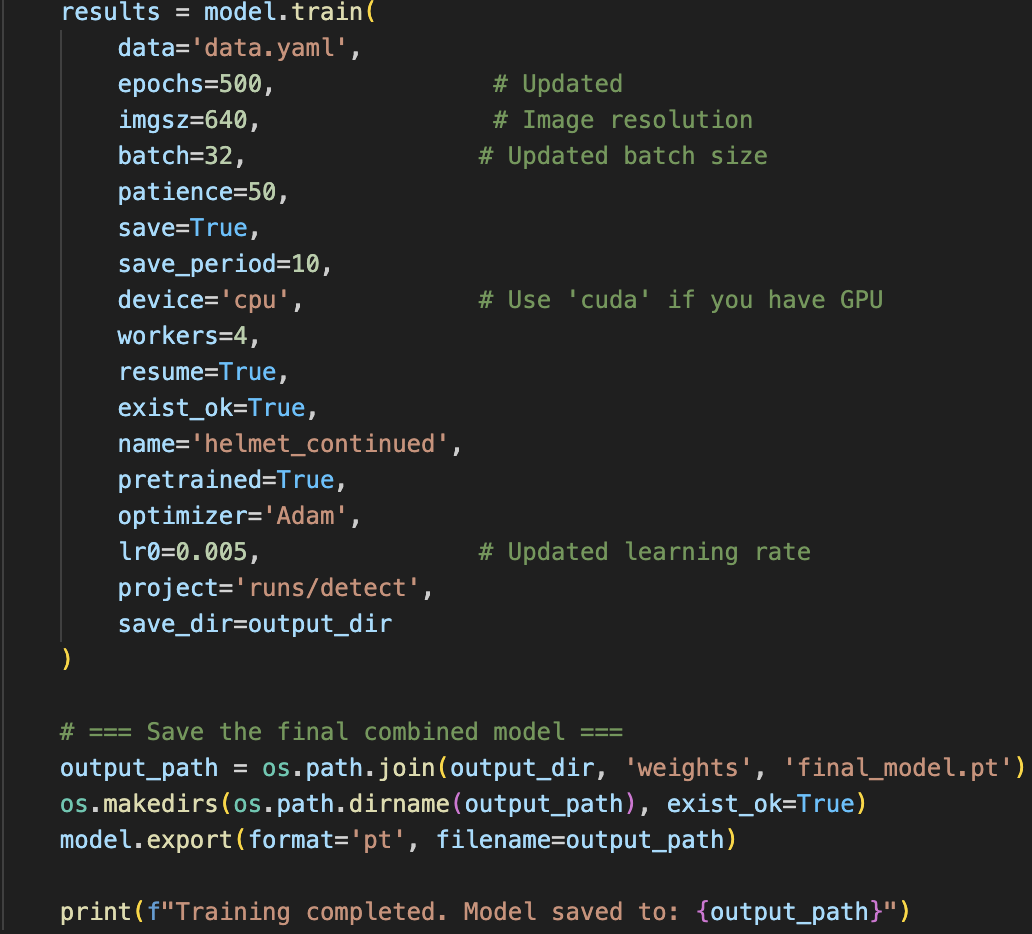
\includegraphics[width=0.8\textwidth]{yaml.png}
	 	
	 	\vspace{0.5em}
	 	\textbf{Figure 3.3.8:  Data.yaml file in VS}
	 \end{center}
\end{itemize}

\section{\textbf{Counting System}}
\subsection{Helmet and Head}

	\noindent\hspace{2.5em}After customizing our YOLOv8 model, we implemented a counting system to track the number of helmets, unhelmeted heads, persons, and motorcycles detected in the video.
	
	
	\noindent\hspace{2.5em}For helmet and head counting, we applied a double-line counting method. This defines a "counting zone" using two vertical lines, and only counts detections whose bounding box centers fall within the zone. To prevent duplicate counting across frames, we used a rolling memory of the last ten frames. If a new detection is within a set distance (e.g., 30 pixels) of a previously counted object of the same type, it is ignored.
	\newline
	This method improves reliability by reducing overcounting and stabilizing results, especially for slow-moving or flickering detections. The final counts are updated in real time and displayed on the video, offering a clear summary of helmet usage and safety compliance.
	\begin{figure}[H] % Optional: [H] requires \usepackage{float}
		\centering
		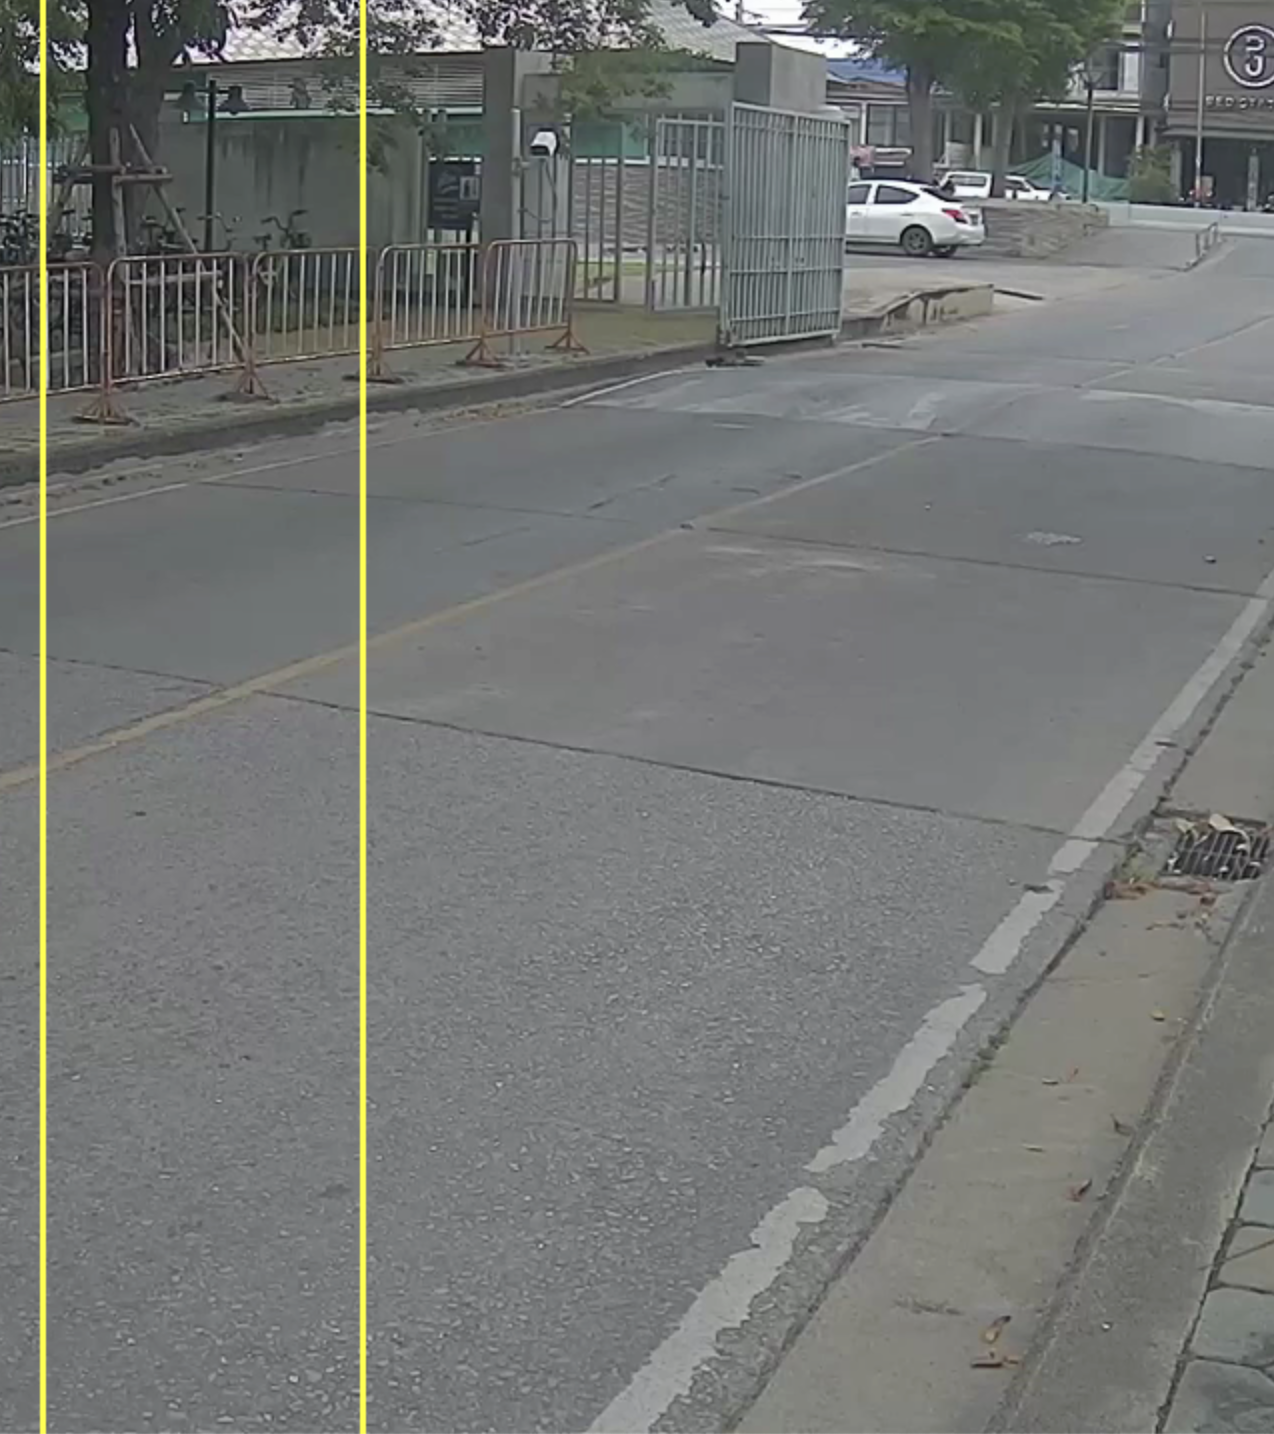
\includegraphics[width=0.5\textwidth]{headhel1.png}
		\vspace{0.5em}
		\caption*{\textbf{Figure 3.2}}
	\end{figure}
	\hfill
	% Right side: Figure 3.3

	\noindent\hspace{2.5em}Figure 3.2 illustrates the designated counting zone used for helmet and head detection. The image shows two vertical yellow lines placed 150 pixels apart, which define the area for double-line counting. When an object passes through both lines in sequence, it is registered as a valid count. This method helps reduce duplicate or false counts caused by temporary detection overlaps or brief tracking loss.
	
	\begin{figure}[H] % Optional: [H] requires \usepackage{float}
		\centering
		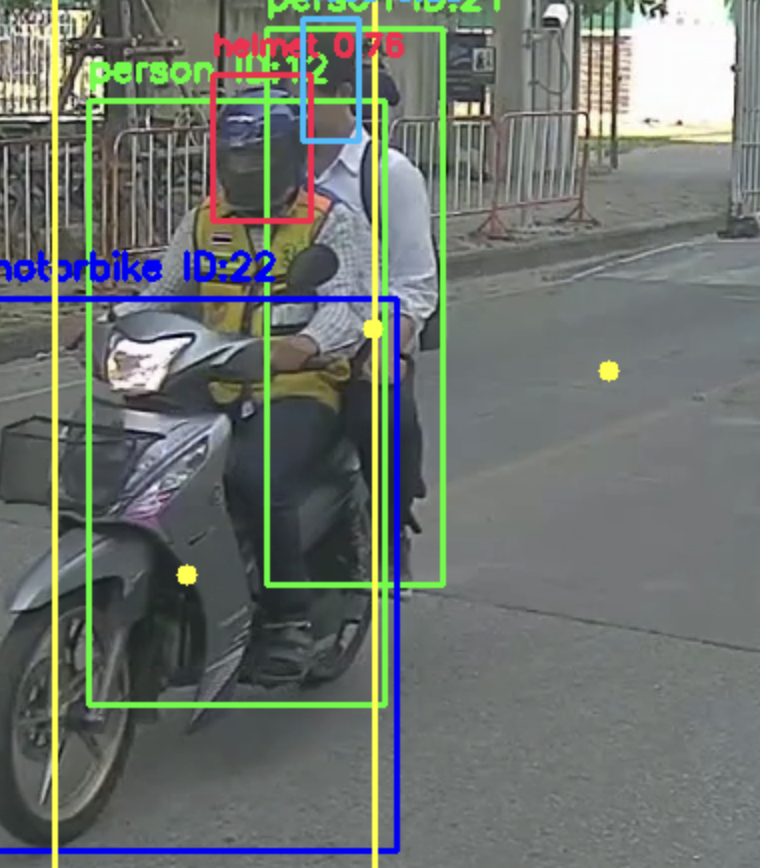
\includegraphics[width=0.5\textwidth]{headhel2.png}
		\vspace{0.5em}
		\caption*{\textbf{Figure 3.3}}
	\end{figure}
	
	\noindent\hspace{2.5em}Figure 3.3 shows an example of the counting system in action when objects, such as a helmet and/or a head, enter the counting zone. As seen in the image, the objects are detected and labeled while passing through the two vertical lines, triggering the counting logic. This illustrates how the system identifies and differentiates helmeted and non-helmeted riders within the defined zone.
	
	\begin{figure}[H] % Optional: [H] requires \usepackage{float}
		\centering
		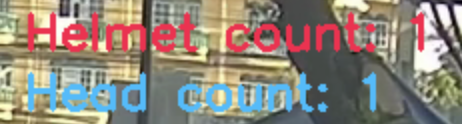
\includegraphics[width=0.5\textwidth]{headhel3.png}
		\vspace{0.5em}
		\caption*{\textbf{Figure 3.4}}
	\end{figure}
	
		\noindent\hspace{2.5em}Figure 3.4 displays the result of the helmet and head counting process, shown at the top-right corner of the screen. These values are updated in real-time after the system detects and counts objects passing through the counting zone. This visual feedback confirms the detection and classification outcome for each rider, distinguishing between helmeted and non-helmeted individuals.
	
	
	
	
\subsection{Person and Motorbike}
\noindent\hspace{2.5em}However as for the Person, and Motorbike detection we can use the Yolov8s.pt model, class 0(person), and class 3(motorbike), as their model are well polished for tracking. For the tracking use Bot-sort tracker, obtain through Roboflow ultralytics/trackers/bot\_sort.py. The tracker will be use to create specific id number for each class that has been detected. Using these id we will create center point of each classes which will be important in the counting method.


\noindent\hspace{2.5em}For the counting method, we can create a region of interest, through using open CV. From there we create a condition, to store the track id with track history. track\_history = {}   function will store the position cx, cy of the tracked object. We will use this value to identify its current and previous position to ensure that when object inside the Region of Interest, position compare is is greater than the current position objected will not be used to count, while if the current position of the tracked id compared to stored id is less than it, it can be counted inside the ROI. This is to ensure that the person, and motorbike can be counted by by what it can be tracked. The detection should look similiar to figure1.

\begin{center}
	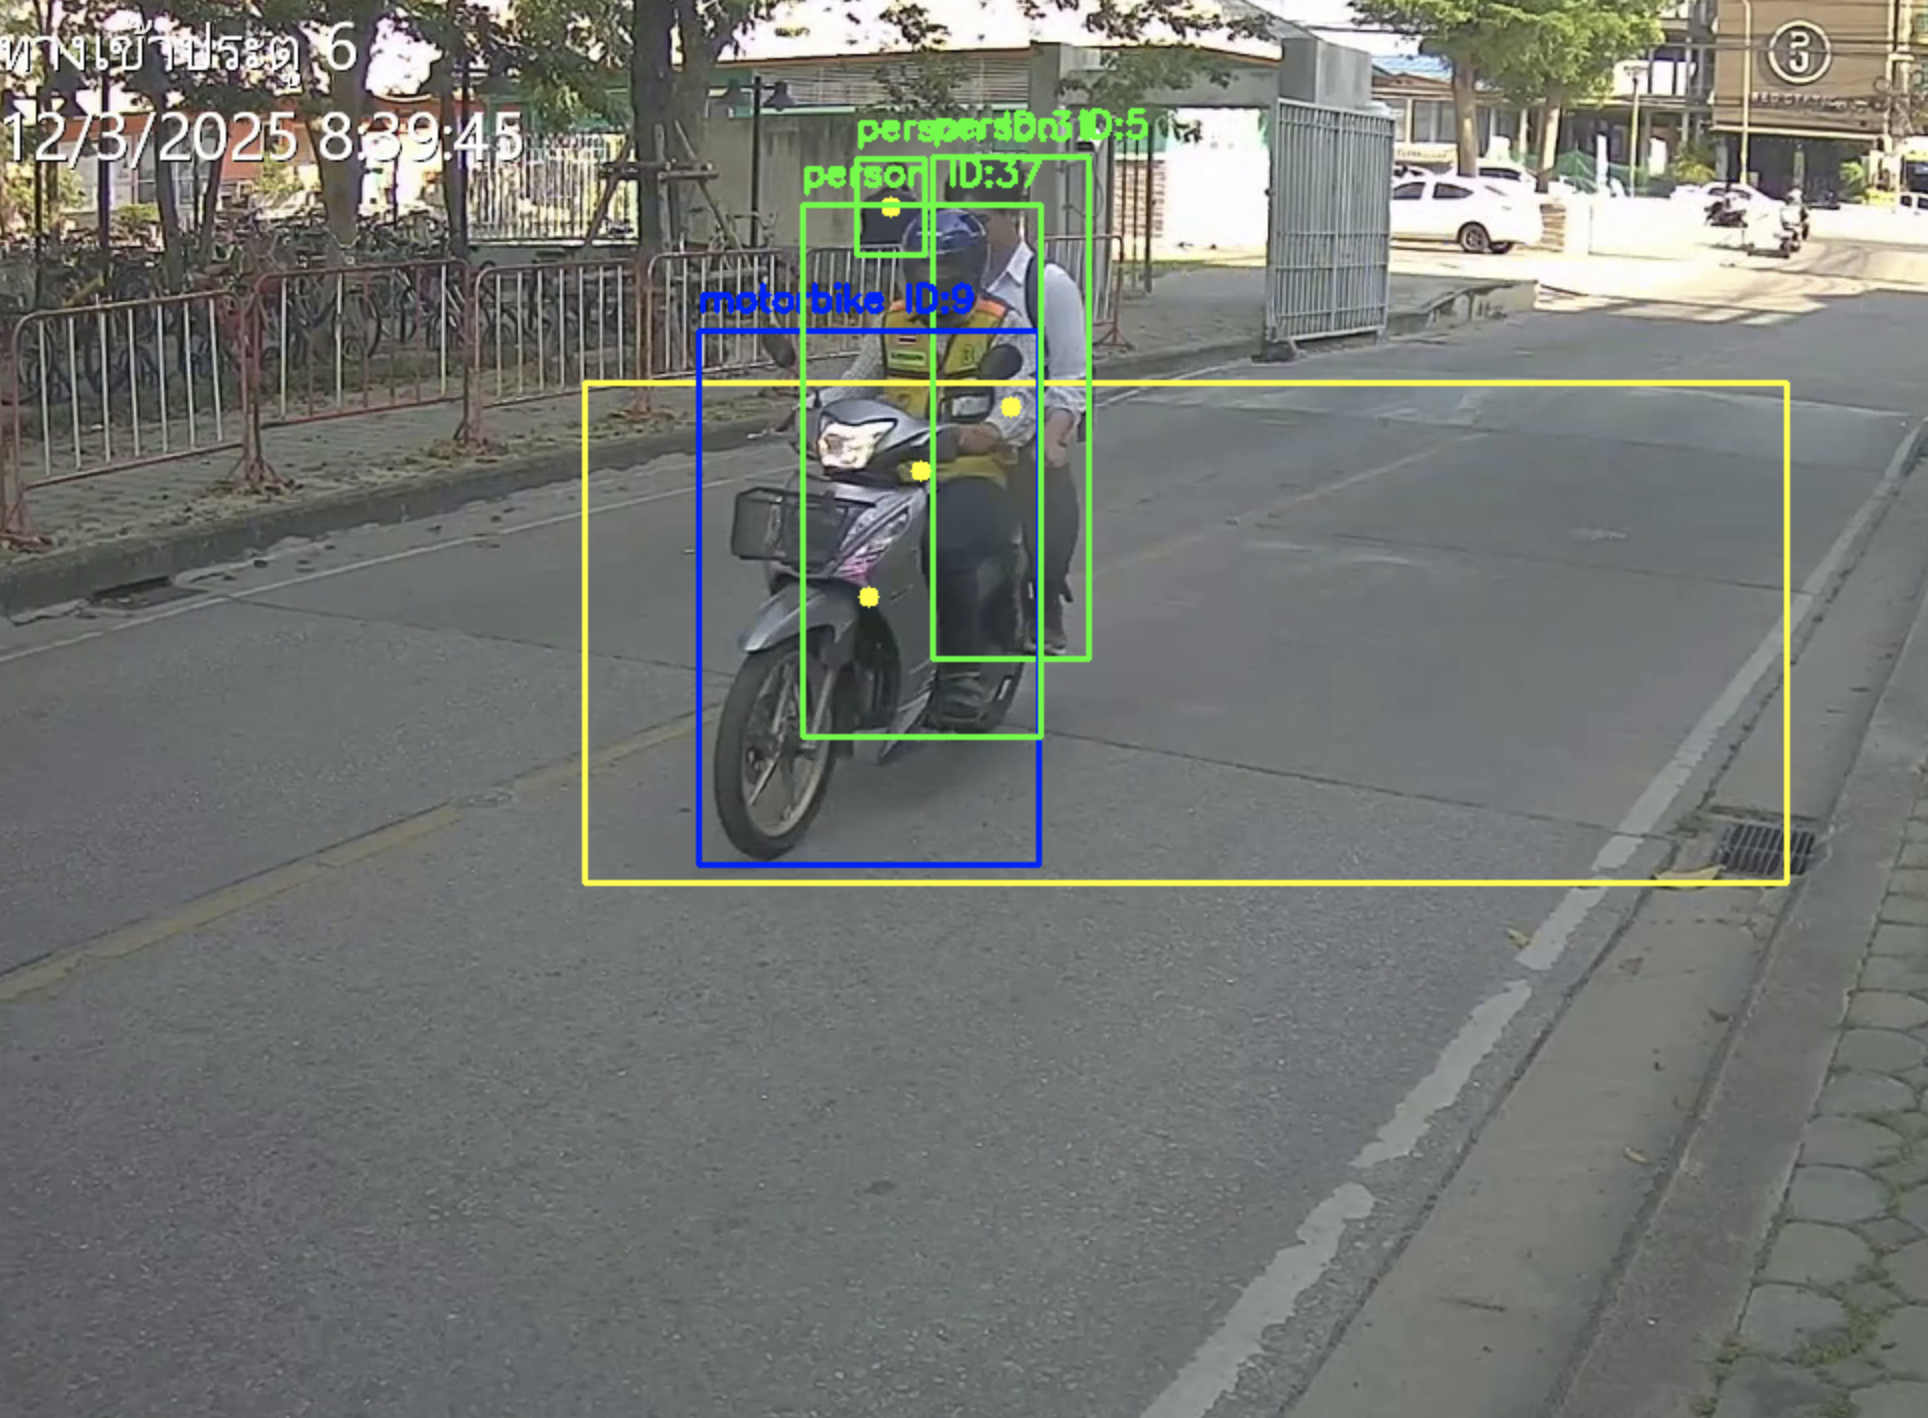
\includegraphics[width=0.5\textwidth]{fig1.png}
	
	\vspace{0.5em}
	\textbf{Figure 3.5}
\end{center}


\subsection{Output Generation}
\noindent\hspace{2.5em}The output generation phase transforms the detection and counting results into a visual and interpretable format. For each processed video frame, the system overlays bounding boxes and labels indicating the object class (helmet, head, person, or motorcycle), along with live counts displayed on the top-left corner using OpenCV. These real-time visual indicators allow users to monitor helmet usage compliance at a glance. Additionally, the system can produce an annotated video file as output, which includes all detections and updated counts across the entire duration. This output is valuable for both immediate observation and later review or reporting, providing a clear and documented summary of safety compliance in the monitored area. The images below shows the output of the system which after we run the program, will show live dection of the video input, and the save video file after the program completed the detection, we save it as a way to easier analyse and observe the detection through video playback, as analysing it live while running maybe not be as efficient.
\begin{center}
	\begin{minipage}{0.45\textwidth}
		\centering
		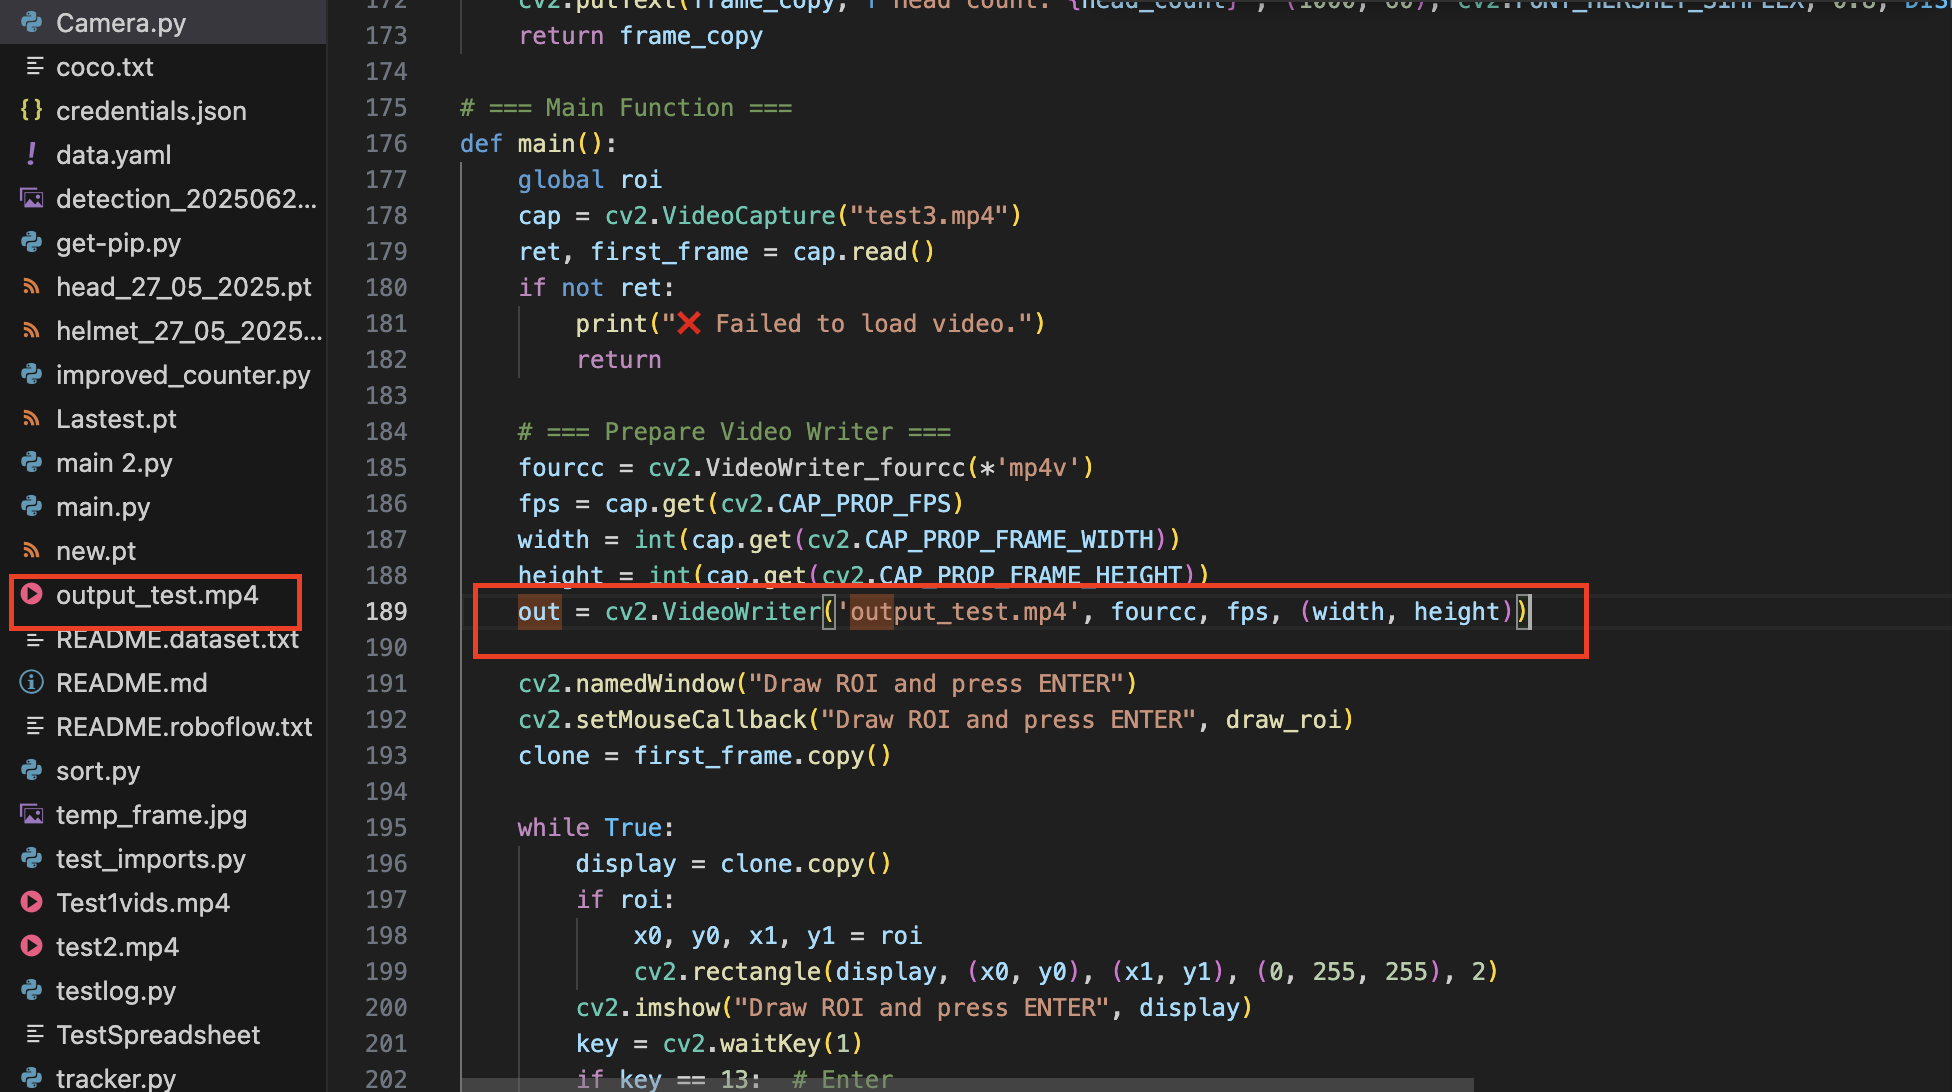
\includegraphics[width=\linewidth]{out.png}
		\vspace{0.7em}
		
		\textbf{Figure 3.4.1: Saved output Video}
	\end{minipage}
	\hfill
	\begin{minipage}{0.45\textwidth}
		\centering
		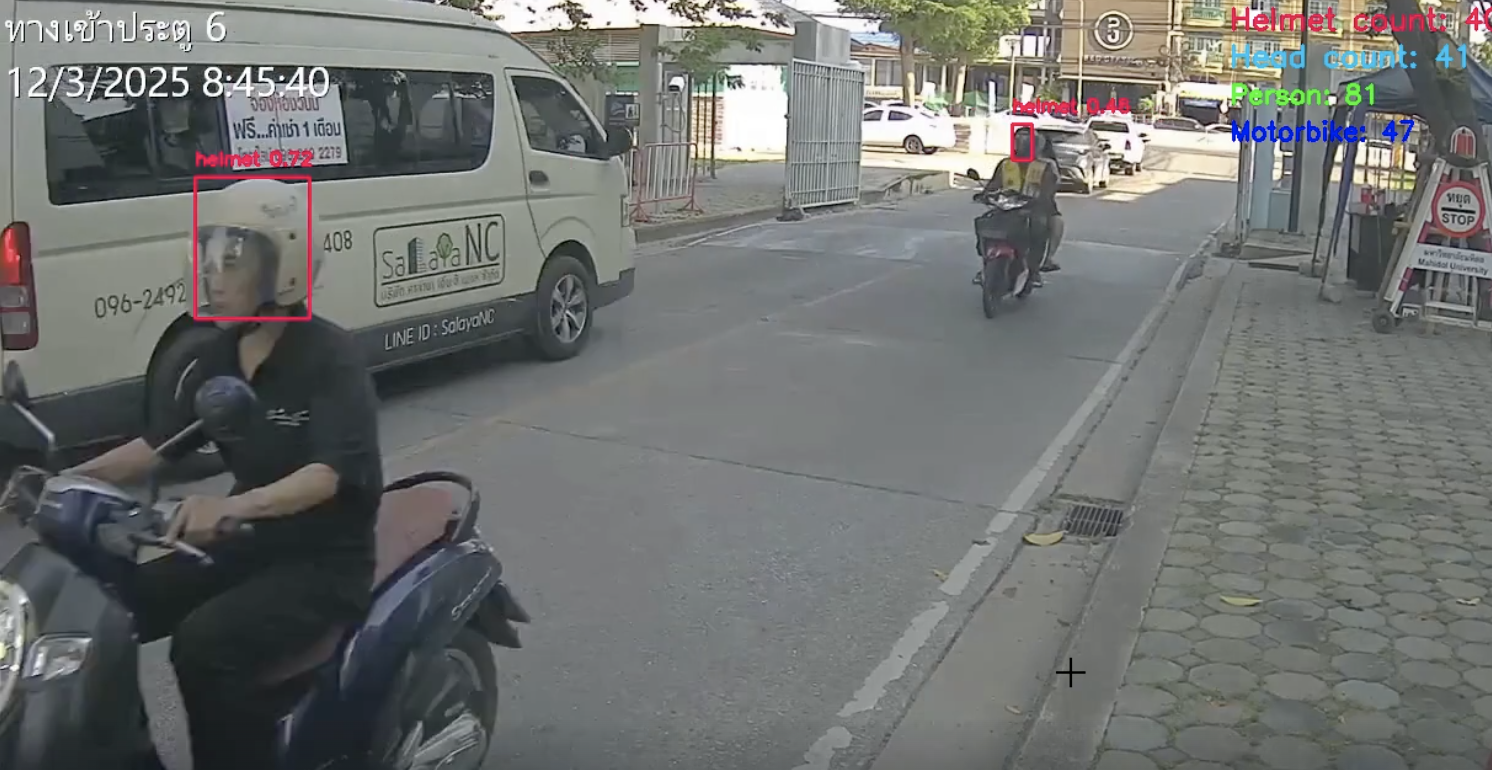
\includegraphics[width=\linewidth]{live.png}
		\vspace{0.5em}
		
		\textbf{Figure 3.4.2: Live Output Generation}
	\end{minipage}
\end{center}


\subsection{Storing Output in Google Sheet API}
\noindent\hspace{2.5em}After the output has been generated, we store the detection into a log using Google API from the video steam. The Google API integration is used for logging and evidence storage for helmet violation cases. Firstly as mention the two model, YOLOv8 pre-trained model, and custom model for head/helmet detection. How the system is works is, when a head is detected within the zone. The frames will be stored, using cv2 to snap-shot the specific frame of head detection. We log the detections events to Google Sheet, it records, the timestamp, head detection, alert, and link to Google Drive file to the captured image.


\noindent\hspace{2.5em}The credentials.json file can be obtained through Google API, the system will connect to pre-defined Google Sheet as we name them(Data log) and appneds the new rows with each detection events that occurs, the image are uploaded to Google Drive using the Drive API, and public access links are generated per log. This implementation allows users to store datas of the detection, this is to allow scalable and automated solution for monitoring helmet violations. The result is as seen in the figure below.

\begin{center}
	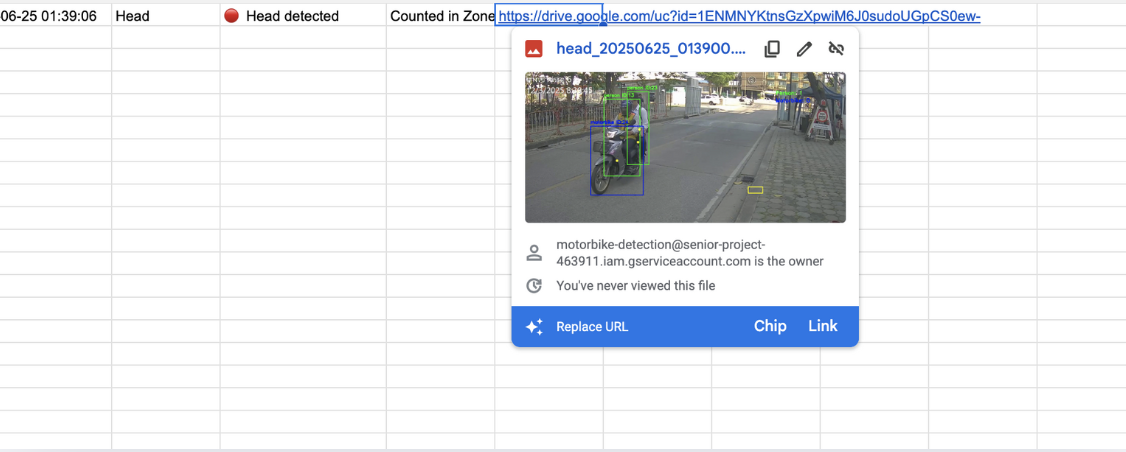
\includegraphics[width=1\textwidth]{api.png}
	
	\vspace{0.5em}
	\textbf{Figure 3.6}
\end{center}

\section{Tools and Frameworks}
\begin{itemize}
	\item \textbf{YOLOv8 Framework}: For object detection.
	\item \textbf{Libraries}: Python libraries such as ultralytics, opencv-python, numpy, collections.
	\item \textbf{Annotation Tools}: Roboflow.
	
\end{itemize}


\section{Hyperparameter Configurations}
During the training process, serveral key herparameters were carefufully selected to balace the performce, the model accuracy and accordingly to our local computation resrouces.

\textbf{Epochs} = 500, this is to ensure suffieicent exposeure to the training datasets. It will allow the model to learn patterns, and improve generalization overtime. However we can stop the early depending on our resources and depending on overfitting.

\textbf{Image Size} imgsz = 640 (image resolution) 640x640 pixel is most commonly use parameter. This will also help decrease the traning time. However for smaller objects like head and helmet detection. Training them on 640x640 is enough, however in some circumstances when training very far, helmet and head that are annotated are risk to losing fine-grained details. This is important as it is very essential for detecting small overlapping objects. For our case we annotate them after they pass the bumper, we have checked that at this area before hand that when resolution was 640x640, it was not too grainy for traing. The image belows shows the annotated image that was resized to 640x640 for training. 


\begin{center}
	\begin{minipage}{0.45\textwidth}
		\centering
		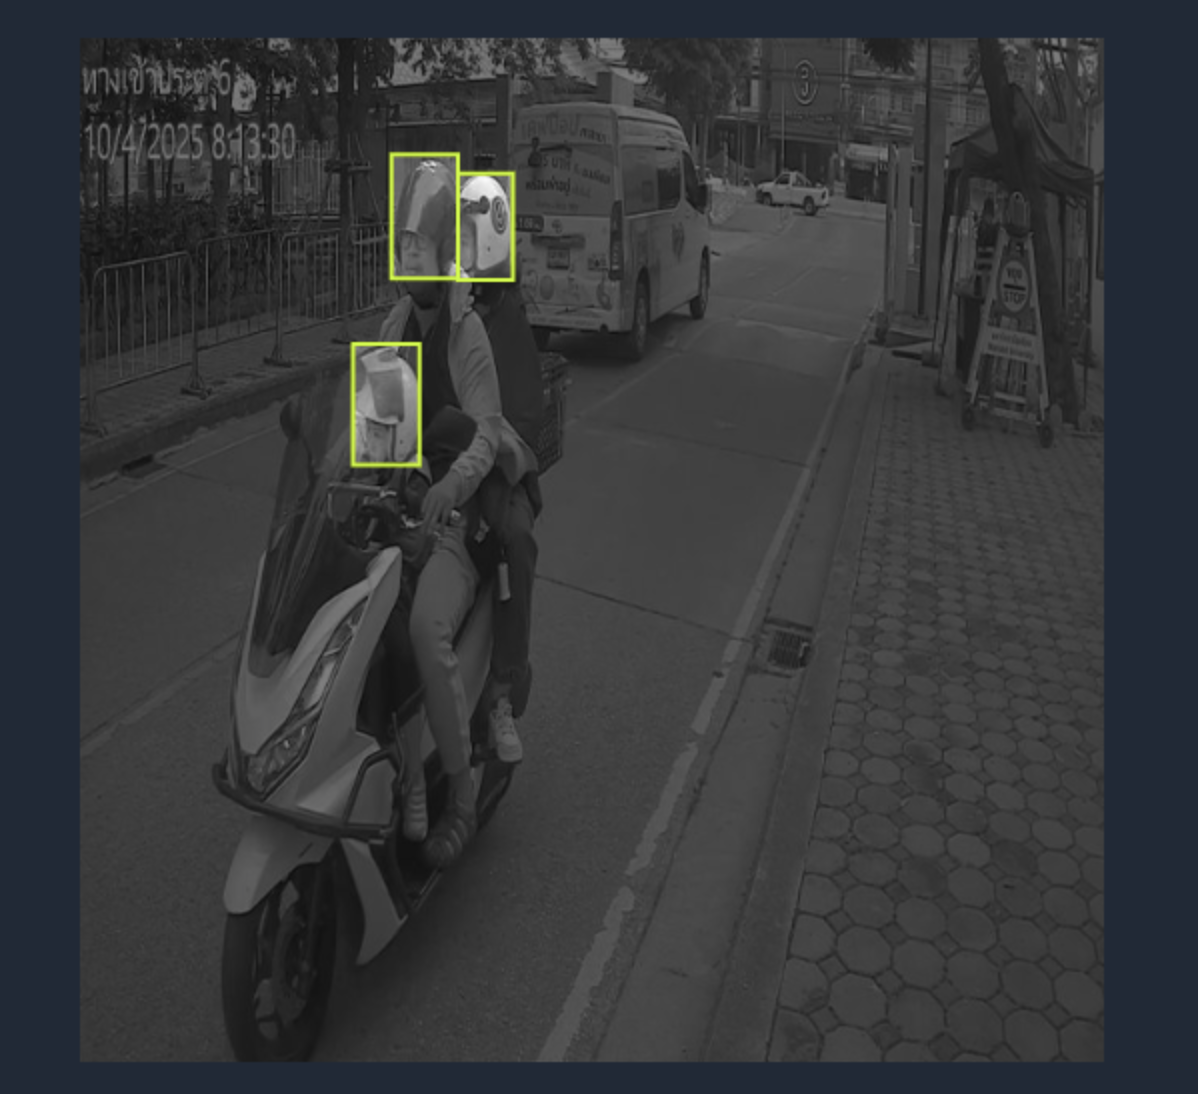
\includegraphics[width=\linewidth]{ano1.png}
		\vspace{0.7em}
		
		\textbf{Figure 3.6.1: Resized Image }
	\end{minipage}
	\hfill
	\begin{minipage}{0.45\textwidth}
		\centering
		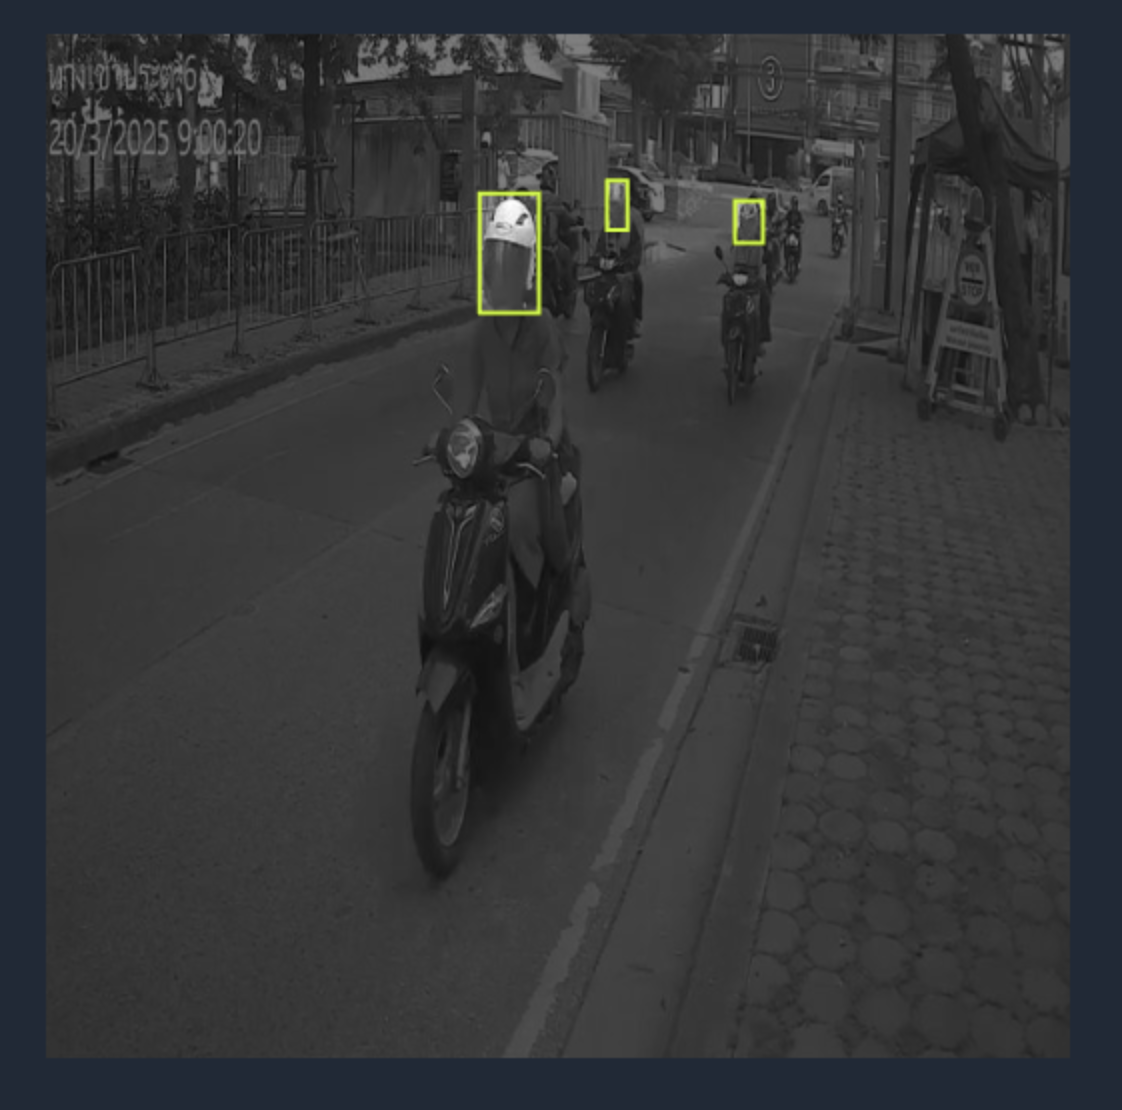
\includegraphics[width=\linewidth]{ano2.png}
		\vspace{0.5em}
		
		\textbf{Figure 3.6.2: Resized Image }
	\end{minipage}
\end{center}




\textbf{Batch Size} =32, this is due to primarily contrained by the GPU, as larger batches can lead larger samples, and faster convergency. Nonetheless, batch size 32istill alowws for reasonable effieicnt traning and consistent model updates. This value can be changed depending on the GPU memory. While a larger batch size could have potentially accelerated training and stabilized gradient updates, our hardware limitations required a compromise at 32 images per batch.

\textbf{Learning Rate} = 0.005. Setting it to this value helps to cacilitate steady learning without causing instability. If it was too high, it could result in model to overshoot the optimal solution during traning. This value is also recommended by YOLOv8.



\section{Performace Evaluation}

\noindent\hspace{2.5em}The trained YOLOv8 model was evaluated using:
mAP: To quantify detection accuracy.
Confusion matrix: To identify true positives, false positives, and negatives.
The purpose of the performance evaluation is to help our team, look at the development of the different models. The benefits of finding the best model is to use them for the best accuracy for the counting systems.

\begin{center}
	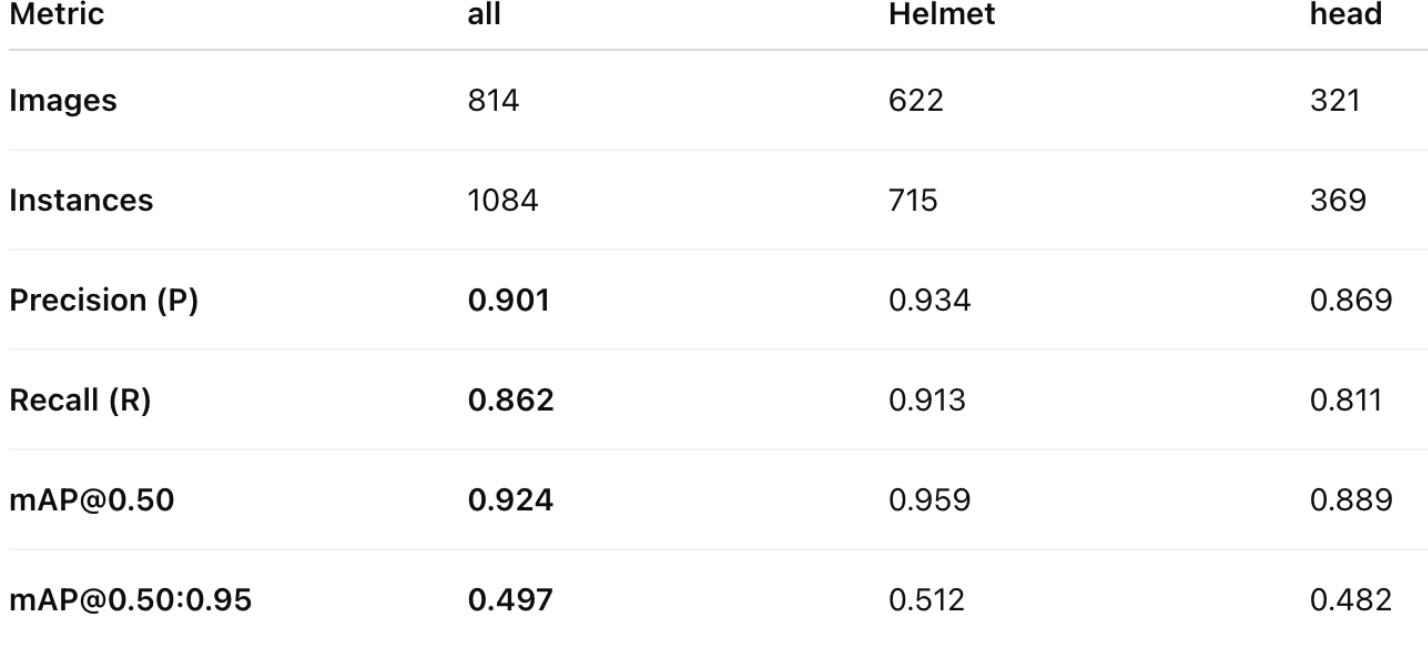
\includegraphics[width=1\textwidth]{performance.eva.png}
	
	\vspace{0.5em}
	\textbf{Figure 3.7}
\end{center}

\noindent\hspace{2.5em}The evaluation results in figure 3.7 demonstrate that the best custom YOLOv8 model performs strongly in detecting both helmet and heads(non-helmet), with particularly high accuracy in helmet detection. Overall, the model achieved a precision of 0.901 and recall of 0.862 across all classes, indicating reliable and consistent predictions. For the helemt class specifically, the model attained satisfying performance with a precision of 0.934, recall of 0.913, and a high mAP@0.50 of 0.959. This suggests that the model can effectively identify helmets with minimal false positives and false negatives. In comparison, the head class yielded slightly lower results, with a precision of 0.869, recall of 0.811, and mAP@0.50 of 0.889, reflecting more variation or complexity in detecting uncovered heads. The overall mAP@0.50:0.95 score of 0.497, while moderate, still indicates acceptable performance under stricter localization conditions. These results affirm the model’s suitability for real-time helmet usage monitoring, particularly in scenarios where accurate helmet detection is critical.

\begin{center}
	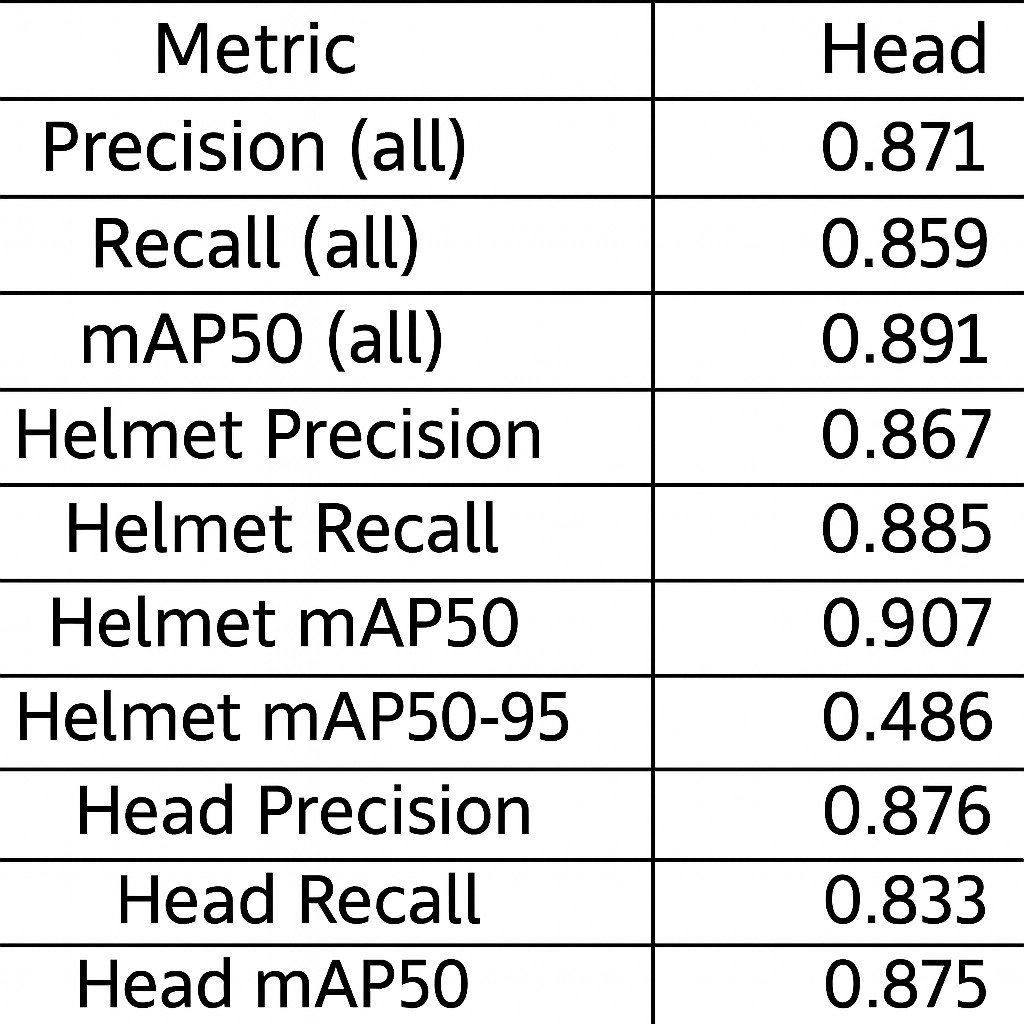
\includegraphics[width=0.5\textwidth]{performance.eva2.png}
	
	\vspace{0.5em}
	\textbf{Figure 3.8}
\end{center}
\noindent\hspace{2.5em}Figure 3.8 shows the previous model performace evaluation, which is call Head\_model. In comparing the performance of the updated helmet and head detection model, which is figure 3.7, to the previous version, several improvements are evident. 

\noindent\hspace{2.5em}The current model achieves an overall precision of 0.901 and recall of 0.862, both higher than the previous model’s precision of 0.871 and recall of 0.859, suggesting better accuracy and detection coverage. Helmet detection has particularly improved, with the current model reaching a helmet precision of 0.934, recall of 0.913, and mAP@0.50 of 0.959, outperforming the previous model’s respective values of 0.867, 0.885, and 0.907. Head detection has also seen slight gains, with the current model achieving 0.869 precision, 0.811 recall, and 0.889 mAP@0.50, compared to 0.876, 0.833, and 0.875 in the earlier version. Additionally, the current model maintains a solid mAP@0.50:0.95 of 0.497 overall, indicating better localization performance under stricter IoU thresholds. These enhancements reflect a more robust and reliable detection system, making the current model better suited for real-world deployment in helmet compliance monitoring scenarios.

	\chapter{RESULT}

\noindent\hspace{2.5em}We have used pre-recorded footage from CCTV cameras to analyze and compare the performance and accuracy of the detection and counting system. 

\vspace{1em}


\section{Model Result}
\noindent\textbf{Table 4.1} \\
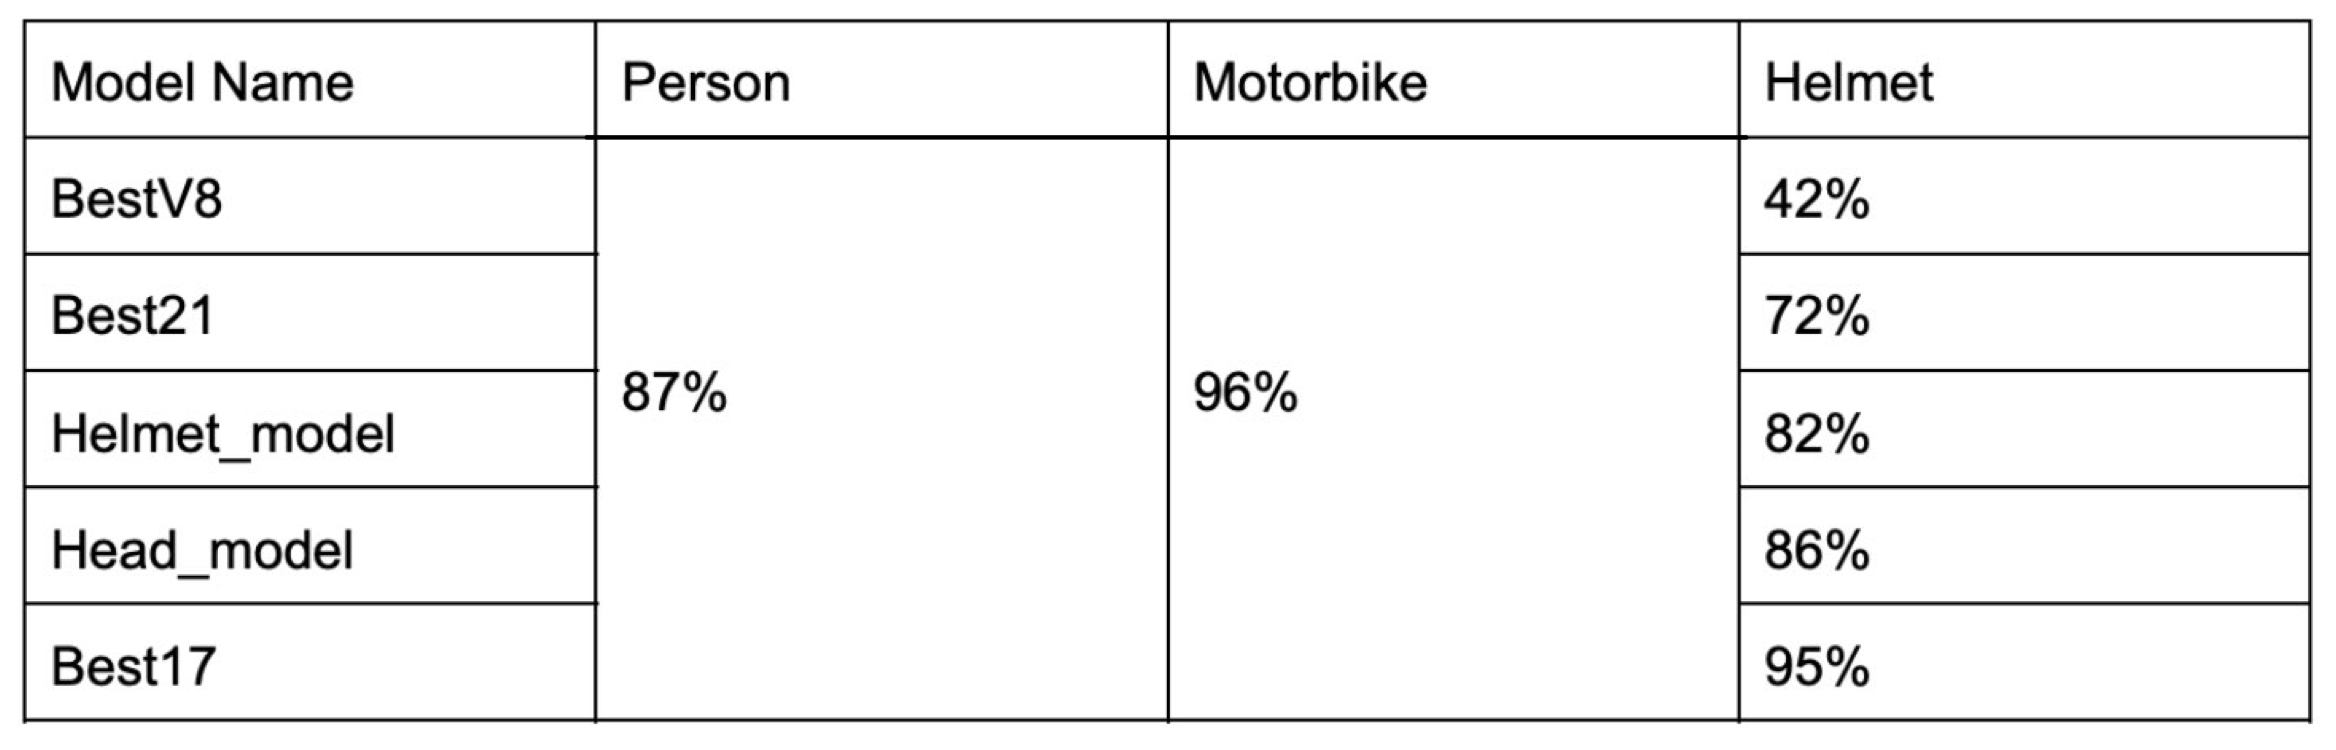
\includegraphics[width=1\textwidth]{table4.1.jpg}


\noindent\hspace{2.5em}To evaluate the accuracy of the model, we compared detection counts with manual counting over a ten-minute span of one video with every model we have. The aim of this is to see the accuracy and improvement of our model. The results in Table 4.1 shows the accuracy results of different models. Person and motorbike used YOLO pretrain model to detect these two classes, so the accuracy and considered constant throughout different models. Helmet detection rises from 42\% to 96\%, which is 54\% improvement from the first model to latest model. The calculation method of finding helemt detection accuracy across different models is to find the total ground truth and detection of the train model, then divide it to find the accuracy. We find the best confident for each model by comparing confident of 0.15 and 0.3 to find the best accuracy. Best17 model have the ground truth helmet of 60, we have the confident set to 0.15 and detected the detection number to be 55, which is 90\%. On the other hand, we change the confident to 0.3 and the results of the detection is 58, which is 95\% resulting in a better accuracy.

Table 4.1 presents the detection accuracy of various models across three object categories: person, motorbike, and helmet. The accuracy values for person and motorbike detection remain constant across models—87\% and 96\% respectively—because these classes were detected using the pretrained YOLO model without additional fine-tuning. In contrast, the helmet detection results vary significantly between models, as each represents a different version of a custom-trained helmet detection model.

\vspace{1em}

\noindent\hspace{2.5em}After evaluating the model's detection accuracy, we proceeded to assess the performance of the counting system. This analysis was conducted using two pre-recorded CCTV footage videos. Tables 4.2 and 4.3 present the counting accuracy for helmeted and non-helmeted (head) riders, derived from Video 1 and Video 2 respectively. These tables utilize a double-line counting method.

\section{Counting Result}
\vspace{0.5em}
\noindent\textbf{Table 4.2} \\
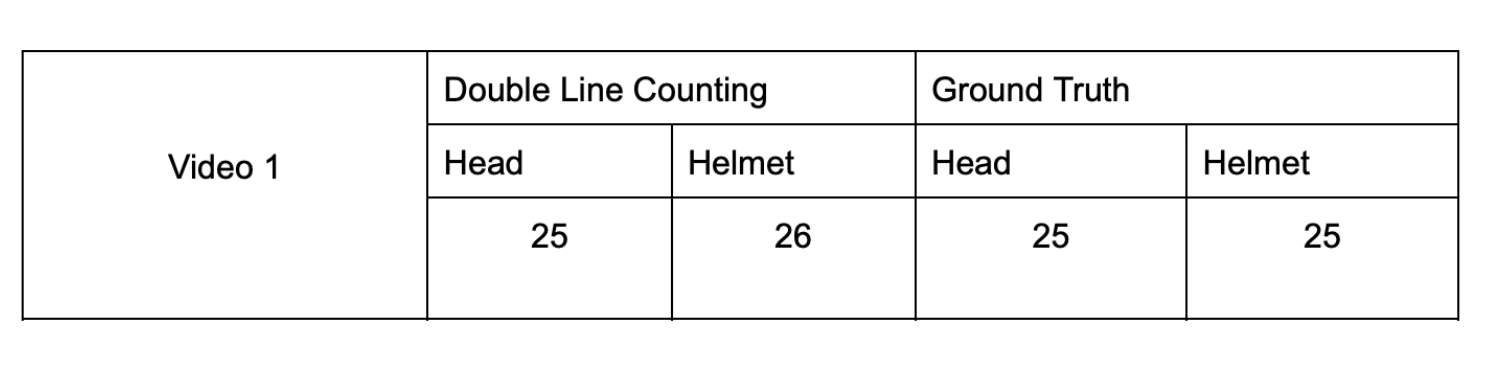
\includegraphics[width=1\textwidth]{test1.png}
\noindent\hspace{2.5em}Table 4.2 shows the counting results for Video 1 using the double-line method compared to the ground truth. The system accurately counted heads (25 vs. 25) but slightly overcounted helmets (26 vs. 25), likely due to duplicate detections or crossing artifacts.


\vspace{0.5em}
\noindent\textbf{Table 4.3} \\
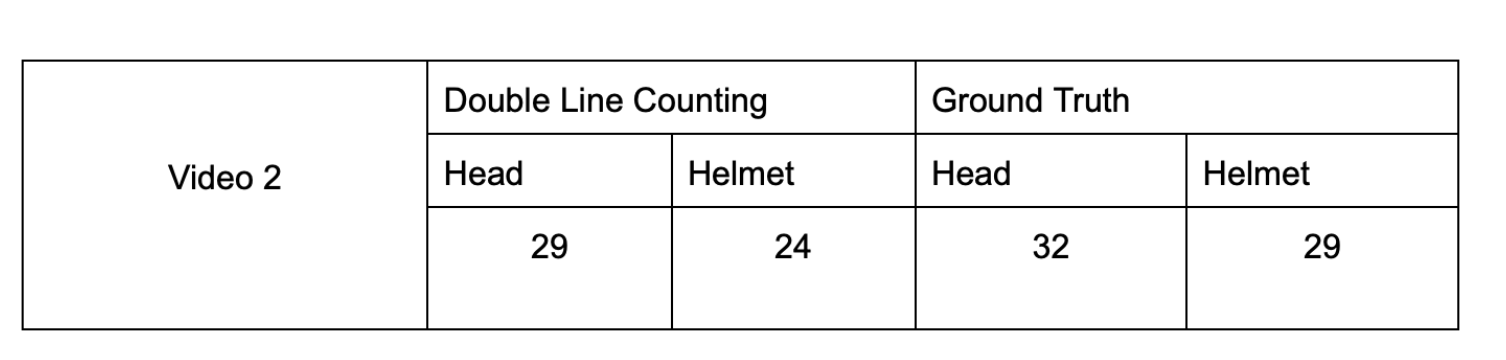
\includegraphics[width=1\textwidth]{test2.png}
\noindent\hspace{2.5em}Table 4.3 shows the double-line counting results for Video 2. The system counted 29 heads and 24 helmets, while the ground truth recorded 32 heads and 29 helmets. This indicates undercounting in both categories, which could be due to missed detections or rapid movements causing objects to skip the counting lines.

\vspace{1em}
For the helmet and head detection specifically, we experimented with adjusting the length of the double-counting lines to evaluate their impact on counting accuracy. For instance, we tested line lengths such as 300 pixels for Line X and 450 pixels for Line Y, along with several other variations. The results indicated that optimal performance occurs when the length of the double lines is kept within approximately 150 pixels. Longer lines tended to increase the likelihood of multiple or false counts due to prolonged object overlap with the counting zone.


\vspace{0.5em}
\noindent\textbf{Table 4.4} \\
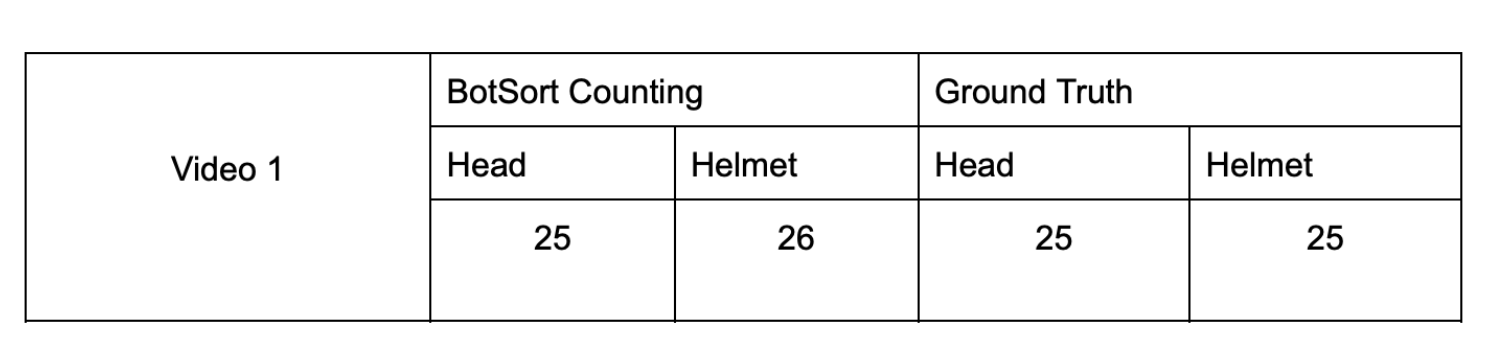
\includegraphics[width=1\textwidth]{test3.png}
\noindent\hspace{2.5em}Table 4.4 presents BotSort counting results for Video 1. The system detected 52 persons and 32 motorbikes, compared to the ground truth values of 51 persons and 30 motorbikes. This reflects a small overcount in both categories, likely due to brief tracking ID switches or overlapping detections in crowded scenes.

\newpage
\vspace{0.5em}
\noindent\textbf{Table 4.5} \\
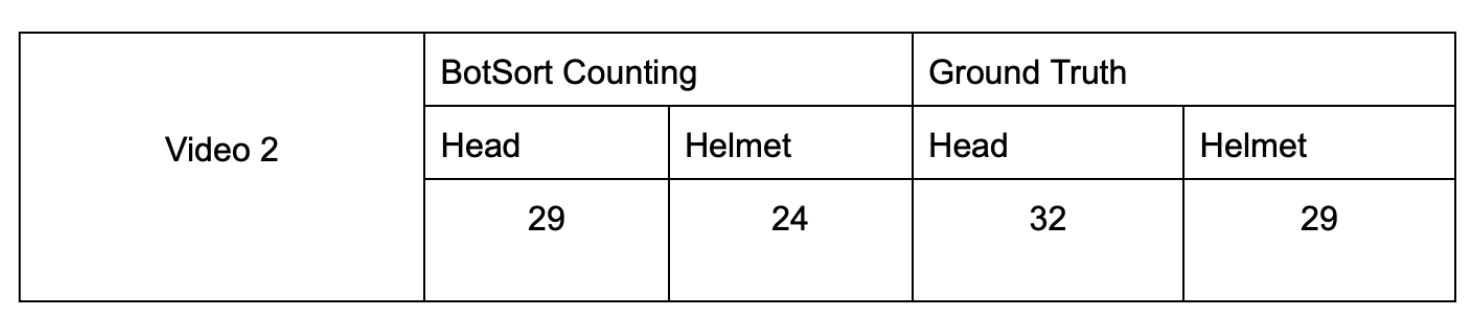
\includegraphics[width=1\textwidth]{test4.png}
\noindent\hspace{2.5em}Table 4.5 summarizes the BotSort results for Video 2. The model counted 56 persons and 44 motorbikes, while the ground truth showed 60 persons and 34 motorbikes. This indicates slight undercounting of persons and significant overcounting of motorbikes, which may result from false positives or tracking drift over longer video durations.


\vspace{1em}
\noindent\hspace{2.5em}In contrast, Tables 4.4 and 4.5 focus on motorbike and person counting accuracy, also based on video 1 and video 2. However, these use the BotSort tracking and counting method instead of the double-line approach. This separation allows us to compare the performance of different counting techniques across differents object categories and scenarios.

\vspace{1em}
\noindent\hspace{2.5em}To evaluate counting accuracy, we use a relative error formula to calculate the percentage difference between the counted value and the ground truth. This approach provides a clear measure of overcounting or undercounting, allowing us to identify and analyze overflow or missed counts in the system.


\vspace{0.5em}
\noindent\textbf{Table 4.6} \\
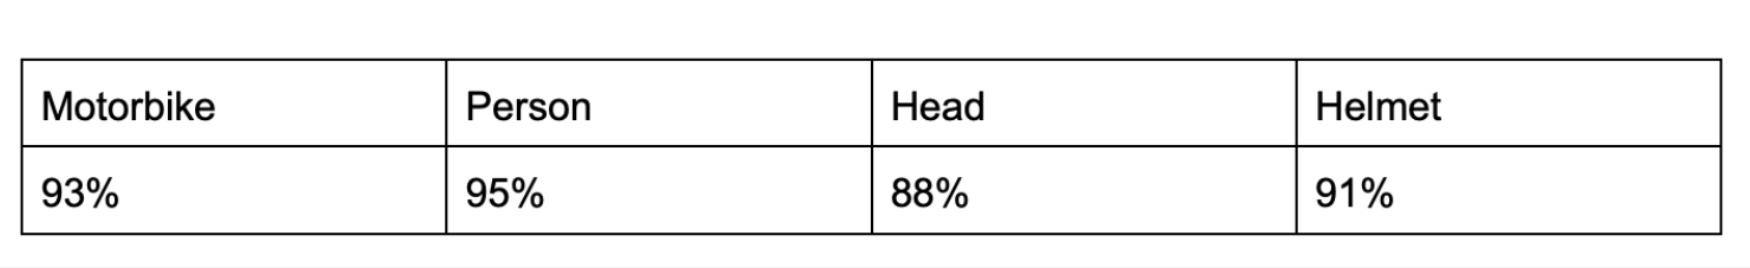
\includegraphics[width=1\textwidth]{conclude_percent.png}

\noindent\hspace{2.5em}Table 4.6 presents the overall performance accuracy of the detection and counting system across four object categories: motorbike, person, head (non-helmeted), and helmet. The results reflect the combined effectiveness of both the object detection model and the counting mechanism (BoT-SORT for motorbike and person, and double-line counting for head and helmet).

The system achieved the highest accuracy in detecting and counting persons (95\%), followed by motorbikes (93\%). These results align with the use of pretrained YOLO models, which provided stable and reliable detection performance. Helmet detection yielded an accuracy of 91\%, demonstrating strong performance from the custom-trained model, especially after multiple iterations and confidence threshold optimization. Head detection (88\%) exhibited slightly lower accuracy, likely due to the challenge of distinguishing non-helmeted heads in varying lighting and occlusion conditions.

Overall, the results confirm that the system performs with high accuracy across all critical object categories, validating its applicability for real-world motorcycle safety monitoring tasks.





	\chapter{Conclusion and Discussion}
\setlength{\parindent}{2.5em}
This project presents a helmet and head detection system trained on a custom dataset using the YOLOv8 architecture, combined with a counting mechanism applied to university CCTV footage. The final model achieved significant accuracy improvements in helmet detection, reaching up to 95\% in our latest version. And applying them to the test videos we have detection average of 91.75\% across all classes detection. Looking at counting methods The double-line counting method effectively reduced duplicate counts and stabilized results, especially for slow-moving or occluded objects. For person and motorbike tracking, the system performed well in low-overlap conditions, providing strong results that demonstrate the system’s potential for practical monitoring and analysis of helmet usage compliance. Additionally we were able to obstecle of counting person, as mentioned there were issues regarding the person detection, as for some cases there were children which are unable to be detected by YOLOv8 pretrained models, another instances such as people overlapping when riding the motor bike, for this case we have switched to combine the count of helmet and head together to total the number of persons. This step is important as be can conclude that our helmet and head detection where accurate enough to combine their count as people. Moreover there where also issues regarding flickering detections for motorbike. For this cases where have used the tracker, and allow the system to store the tracker location and ID through track\_history. This function allows us to compare the possition of the previous detection and the new detection. This is to make sure that the tracker rememebers the movement of the object it is tracking. The counting for the motorbike is done solely based on the tracker's center point of the bouding boxes and comparing the ID history position with the current position to help aid with the Bot\_sort Tracker. This method works well with the YOLOv8 pretrained model for motorbike detection, simply we were able to find a Region of Interest so that we do not also count motor bike and people going out of the scene. 


\section{Obstacles}

\begin{center}
	\begin{minipage}{0.45\textwidth}
		\centering
		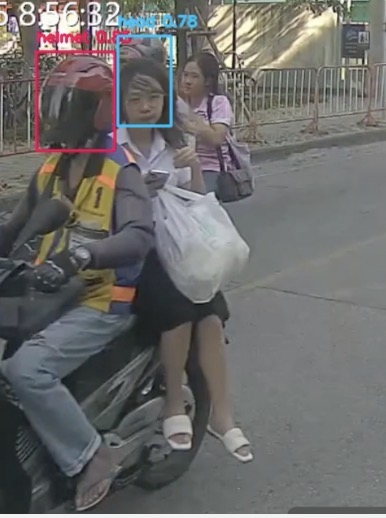
\includegraphics[width=\linewidth]{limitation2.png}
		\vspace{0.5em} % Adjust as needed
		
		\textbf{Figure 5.1}
	\end{minipage}
	\hfill
	\begin{minipage}{0.45\textwidth}
		\centering
		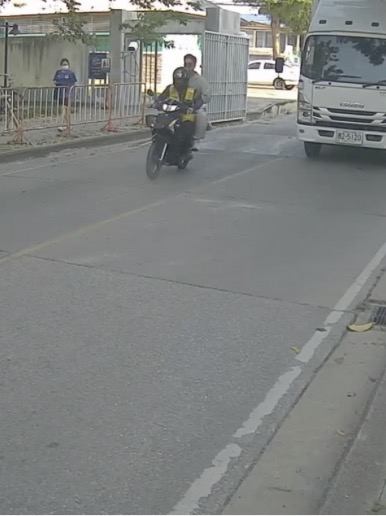
\includegraphics[width=\linewidth]{limitation3.png}
		\vspace{0.5em} % Match the first one
		
		\textbf{Figure 5.2}
	\end{minipage}
\end{center}
\setlength{\parindent}{2.5em}
During system development and testing, the main challenge involved dealing with overlapping bounding boxes, particularly when multiple motorcycles and riders appeared close together. This sometimes led to incorrect object counts or detection errors, such as merging two people into one or misidentifying a detection. The tracking system also struggled when many objects entered the counting zone at once, occasionally creating new IDs for the same object however we uses Bot\_sort Tracker to help minimize the flickering as possible, as when they enter the counting zone, if object is redetected there are chances new ID will appear and our system could not reidentify the object, it would count that object base on the new ID.

These issues were more pronounced in crowded scenes and highlight the limitations of relying on bounding box-based tracking in complex real-world environments. which can be seen in Figure 5.1. This sometimes led to incorrect object counts or detection errors, because there are another object blocking another object in the counting zone. 

In Figure 5.2 another flaw showing the struggle of tracking system when an object appear to be on another lane, causing it hard for our model to detect an object, especially when it appear to far from the annotation point. 


\section{Future Work}
\setlength{\parindent}{2.5em}
In future iterations, the focus will be on improving both the detection model and the tracking accuracy. Training with more diverse and balanced data will help the model generalize better across various environments and video conditions. Further enhancement of the counting and tracking logic is also planned to address issues with ID switching and occlusion. Additionally, while deployment to the university server is not yet complete, it remains a key objective for real-time monitoring in a practical setting. These improvements will support the goal of developing a more accurate, stable, and scalable helmet compliance monitoring system.




	\newpage
	%---- Bibliography -----
	\pagestyle{bibliography}
	\bibliography{references} 
	\bibliographystyle{abbrvnat}
	\label{lastpage}
	\newpage
	%---- Appendix ----
	%\coverAppendix
	%\pagestyle{appendix}
	%\appendix
	%\chapter{TEST APPENDICES}

Node.js is an open source and cross platform JavaScript runtime environment [5]. Node.js allows developers to use JavaScript to write the command line tools and for server-side scripting to produce dynamic web page content before the page publishes to the users’ web browser.

\section{Figure}
Node.js is an asynchronous event-driven JavaScript runtime which is designed to build scalable network applications. It runs with the V8 JavaScript engine outside of the browser. Therefore, Node.js becomes very performant.

\begin{figure}[htbp]
    \centering
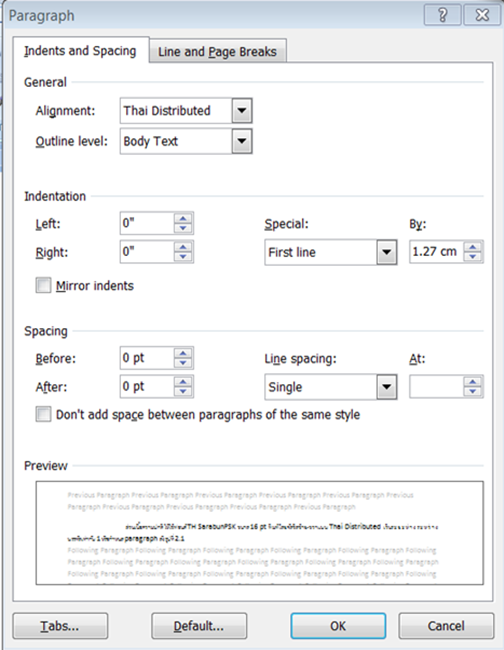
\includegraphics[width = 0.5\textwidth]{paragraph.png}
    \caption{Paragraph arrangement}
    \label{fig:paragraph}
\end{figure}

\subsection{Equation}
Node.js is an asynchronous event-driven JavaScript runtime which is designed to build scalable network applications. It runs with the V8 JavaScript
\begin{equation}
E=mc^{2}
\end{equation}
นิยมวางสมการไว้กึ่งกลางหน้ากระดาษ และหมายเลขสมการพิมพ์ชิดขวา

\subsubsection{Coding}
Node.js is an asynchronous event-driven JavaScript runtime which is designed to build scalable network applications. It runs with the V8 JavaScript 

\begin{lstlisting}[language=C]
public static void main(String[] args)
{
	System.out.println(“Hello World”);
}
\end{lstlisting}
\section{Table}
GraphQL is both an API query language and a runtime for executing those queries using your current data. GraphQL allows clients the power to ask for exactly what they need and nothing more, makes it easier to evolve APIs over time, and enables powerful developer tools by providing a clear and intelligible description of the data in your API
\begin{table}[hbt!]
    \caption{ตารางข้อมูลตัวอย่าง}
    \centering
    \begin{tabularx}{\textwidth}{|Y|Y|Y|Y|}
    \hline
       ลำดับที่ & ตัวแปร & ค่าของตัวแปร & ตัวอย่าง  \\
    \hline
        1 & $x$ & 15 & $x=15$\\
    \hline
        2 & $y$ & 30 & $y=30$\\
    \hline
    \end{tabularx}
    \label{tab:my_label}
\end{table}

\subsection{Equation}
Node.js is an asynchronous event-driven JavaScript runtime which is designed to build scalable network applications. It runs with the V8 JavaScript
\begin{equation}
E=mc^{2}
\end{equation}
นิยมวางสมการไว้กึ่งกลางหน้ากระดาษ และหมายเลขสมการพิมพ์ชิดขวา

\subsubsection{Coding}
Node.js is an asynchronous event-driven JavaScript runtime which is designed to build scalable network applications. It runs with the V8 JavaScript 

\begin{lstlisting}[language=C]
public static void main(String[] args)
{
	System.out.println(“Hello World”);
}
\end{lstlisting}
\section{Table}
GraphQL is both an API query language and a runtime for executing those queries using your current data. GraphQL allows clients the power to ask for exactly what they need and nothing more, makes it easier to evolve APIs over time, and enables powerful developer tools by providing a clear and intelligible description of the data in your API
\begin{table}[hbt!]
    \caption{ตารางข้อมูลตัวอย่าง}
    \centering
    \begin{tabularx}{\textwidth}{|Y|Y|Y|Y|}
    \hline
       ลำดับที่ & ตัวแปร & ค่าของตัวแปร & ตัวอย่าง  \\
    \hline
        1 & $x$ & 15 & $x=15$\\
    \hline
        2 & $y$ & 30 & $y=30$\\
    \hline
    \end{tabularx}
    \label{tab:my_label}
\end{table}
	
\end{document}